\documentclass{sig-alternate}
\setlength{\paperheight}{11in}
\setlength{\paperwidth}{8.5in}
% these packages must be loaded in this order, and before any other packages
\usepackage[utf8]{inputenc}
\usepackage[T1]{fontenc}
\usepackage[final]{microtype}
% these packages must be loaded in this order
\usepackage[nocompress]{cite}
\usepackage[hyphens]{url}
\usepackage{color}
\usepackage{hyperref}
\hypersetup{colorlinks=true,urlcolor=blue,citecolor=dgreen,
            pageanchor=false,pdfpagelabels=false}
% CCS printer wants link colors disabled
\hypersetup{hidelinks=true}
% the order of the rest of these packages does not matter, so they're
% sorted alphabetically
\usepackage{authblk}
\usepackage{booktabs}
\usepackage[margin=10pt,font=small,labelfont=bf]{caption}
\usepackage[font=small]{subcaption}
\DeclareCaptionType{copyrightbox}%fix caption/sig-alternate compat issue
\usepackage{comment}
\usepackage{listings}
\usepackage{paralist}
\usepackage{siunitx}
\usepackage{tikz}
\usepackage[l2tabu,orthodox]{nag}
%
\definecolor{dgreen}{RGB}{0,127,0}
\pgfrealjobname{stegotorus}
\usetikzlibrary{arrows}
\usetikzlibrary{decorations.pathmorphing}
% siunitx 2.0 renamed all the options, feh
% we only need the bit and byte units, not the binary prefixes
\makeatletter
\@ifpackagelater{siunitx}{2011/06/15}
  {\sisetup{per-symbol=/,per-mode=symbol,group-separator={,},
            range-units=single}
   \DeclareSIUnit{\bit}{bit}
   \DeclareSIUnit{\byte}{B}}
  {\sisetup{per=slash,digitsep=comma,trapambigrange=false}
   \newunit{\bit}{bit}
   \newunit{\byte}{B}}
\makeatother
% \SI shorthands
\newcommand{\kbps}[1]{\SI{#1}{\kilo\bit\per\second}}
\newcommand{\Mbps}[1]{\SI{#1}{\mega\bit\per\second}}
\newcommand{\kBps}[1]{\SI{#1}{\kilo\byte\per\second}}
\newcommand{\msec}[1]{\SI{#1}{\milli\second}}
%
\hyphenation{white-list-ing ad-ver-sar-ies anon-y-mized}
\lstset{basicstyle=\fontfamily\ttdefault\fontsize{6.5}{7}\selectfont,
        xleftmargin=7pt,morecomment=[s]{<}{>}}
\DeclareTextFontCommand{\textitt}
  {\fontfamily\ttdefault\fontshape\itdefault\selectfont}
%\renewcommand{\baselinestretch}{0.975}
%
\bibliographystyle{acmurl}
%
\makeatletter
\def\@openbib@code{}
\newcommand*{\BIBdecl}{%
  % cribbed from biblatex 1.7; / moved from Breaks to BigBreaks to
  % ensure that 'http://' is not broken after the colon
  \Urlmuskip=0mu plus 3mu\relax
  \mathchardef\UrlBigBreakPenalty=100\relax
  \mathchardef\UrlBreakPenalty=200\relax
  \def\UrlBigBreaks{\do\:\do\-\do\/}%
  \def\UrlBreaks{%
    \do\.\do\@\do\\\do\!\do\_\do\|\do\;\do\>\do\]\do\)\do\}%
    \do\,\do\?\do\'\do\+\do\=\do\#\do\$\do\&\do\*\do\^\do\"}%
}
% Make affiliations all on one line, fix the apparent ordering
% of commas and footnote marks, and apply ACM's font choices.
\renewcommand\AB@affilsepx{\qquad\protect\Affilfont}
\renewcommand\AB@authnote[1]
    {\rlap{\lower-0.4em\hbox{\kern0.7pt\relax%
      \fontfamily{txss}\fontsize{8}{9}\selectfont #1}}}
\renewcommand\AB@affilnote[1]
    {\leavevmode\lower-0.4em\hbox{\kern-0.5pt\relax%
      \fontfamily{txss}\fontsize{7}{8}\selectfont #1}}
\renewcommand\Authsep{,\hskip 8.5pt\relax}
\renewcommand\Authands{,\hskip 5.5pt\relax and~}
\renewcommand\Authfont{\aufnt}
\renewcommand\Affilfont{\affaddr}
\makeatother
%
\begin{document}

% annotations for the first page of the camera-ready
\conferenceinfo{CCS'12,} {October 16--18, 2012, Raleigh, North Carolina, USA.}
\CopyrightYear{2012}
\crdata{978-1-4503-1651-4/12/10}
\clubpenalty=10000
\widowpenalty=10000

\title{StegoTorus: A Camouflage Proxy for the Tor Anonymity System}

\author[1,2]{Zachary~Weinberg}
\author[3]{  Jeffrey~Wang}
\author[2]{Vinod~Yegneswaran}
\author[2]{Linda~Briesemeister}
\author[2]{Steven~Cheung}
\author[3]{Frank~Wang}
\author[3]{Dan~Boneh}

\affil[1]{Carnegie~Mellon~University}
\affil[2]{SRI~International}
\affil[3]{Stanford~University}

\maketitle

Studies of Internet censorship rely on an experimental technique
called \textit{probing}.  From a client within each country under
investigation, the experimenter attempts to access network resources
that are suspected to be censored, and records what happens.  The set
of resources to be probed is a crucial, but often neglected, element of the
experimental design.

We analyze the content and longevity of 758,191 webpages drawn from 22
different probe lists, of which 15 are alleged to be actual blacklists
of censored webpages in particular countries, three were compiled using
\emph{a~priori} criteria for selecting pages with an elevated chance
of being censored, and four are controls.  We find that the lists have
very little overlap in terms of specific pages.  Mechanically
assigning a topic to each page, however, reveals common themes, and
suggests that hand-curated probe lists may be neglecting certain
frequently-censored topics.  We also find that pages on controversial
topics tend to have much shorter lifetimes than pages on
uncontroversial topics.  Hence, probe lists need to be continuously
updated to be useful.

To carry out this analysis, we have developed automated infrastructure
for collecting snapshots of webpages, weeding out irrelevant material
(e.g.\ site “boilerplate” and parked domains), translating text,
assigning topics, and detecting topic changes.  The system scales to
hundreds of thousands of pages collected.

\section{Introduction}\label{s:intro}

Freedom of speech and decentralization are bedrock principles of the
modern Internet.  John Gilmore famously said that “the Net interprets
censorship as damage, and routes around it”~\cite{q-gilmore}.  It is
more difficult for a central authority to control what is published on
the Internet than on older, broadcast-based media; in 2011, the
Internet's utility to the “Arab Spring” revolutions prompted a
spokesman for the US Department of State to label it “the Che Guevara
of the 21st century”~\cite{q-ross}.  Nonetheless, national governments
can easily inspect, manipulate, and block nearly all network traffic
that crosses their borders. Over a third of all nations impose
“filters” on their citizens' view of the Internet~\cite{n-global}.  As
the Internet continues to grow in scope and importance, we can expect
that governments will only increase their efforts to control
it~\cite{q-celine}.

Tools for evading online censorship are nearly as old as the
censorship itself~\cite{c-peacefire,c-howto-book}.  At present, one of
the most effective circumvention tools is “Tor”~\cite{c-tor}.  Tor
provides anonymity for its users by interposing three relays between
each user and the sites that the user visits.  Each relay can decrypt
just enough of each packet to learn the next hop. No observer at any
single point in the network, not even a malicious relay, can know both
the source and the destination of Tor traffic.

Although Tor was not designed as an anticensorship tool, it works well
in that role.  Repressive governments respond by blocking Tor
itself. In 2010 and 2011, Iran attempted to block Tor traffic by
scanning TLS handshakes for Diffie-Hellman parameters and/or
certificate features that were characteristic of
Tor~\cite{n-iran1,n-iran2}.  China employed a similar technique but
enhanced it with active probing of the suspected Tor relay, mimicking
the initial sequence of Tor protocol messages in
detail~\cite{n-china-active}.  The Tor developers defeated these
blocks with small adjustments to their software.

For a few days in early 2012, Iran blocked \emph{all} outbound HTTPS
connections to many websites~\cite{n-iran3}, including Tor's primary
site.\footnote{\url{https://www.torproject.org/}} To evade this more
drastic blockade, Tor deployed a program called \textit{obfsproxy}
(for “obfuscating proxy”)~\cite{n-iran-ob}.  Obfsproxy applies an
additional stream cipher to Tor's traffic.  This frustrates any filter
looking for a specific plaintext pattern (such as a TLS handshake),
but does not significantly alter packet sizes and timing.  As we will
discuss in Section~\ref{s:detect-tor}, this means that Tor is still
easily fingerprintable.

\smallskip\noindent\textbf{Contributions:} In this paper, we present
an elaboration on the obfsproxy concept, StegoTorus.  StegoTorus
currently consists of:
\begin{compactitem}
\item A generic architecture for concealing Tor traffic within an
  innocuous “cover protocol” (Section~\ref{s:arch}).
\item A novel encrypted transport protocol geared specifically for the
  needs of steganography (Section~\ref{s:chop}).
\item Two proof-of-concept steganography modules (Section~\ref{s:steg}).
\end{compactitem}
We will demonstrate the ease of detecting un-camouflaged Tor traffic
and StegoTorus' effectiveness at concealing it, even with the current
proof-of-concept steganography (Sections~\ref{s:detect-tor}
and~\ref{s:detect-fb}).  We will also demonstrate that StegoTorus
imposes a reasonable amount of overhead for what it does
(Section~\ref{s:peval}).

We anticipate that censors will adapt quickly to this advance on the
circumvention side of the arms race; more sophisticated and varied
steganography modules are under active development.  Ultimately, an
attacker will need to defeat \emph{all} of the steganography modules
used by StegoTorus to block Tor traffic.

%% Creator: Inkscape inkscape 0.48.3.1, www.inkscape.org
%% PDF/EPS/PS + LaTeX output extension by Johan Engelen, 2010
%% Accompanies image file 'arch.pdf' (pdf, eps, ps)
\begingroup%
  \setlength{\unitlength}{209.6bp}%
  \fontsize{7pt}{7pt}\selectfont
  \begin{picture}(1,0.8325522)%
    \put(0,0){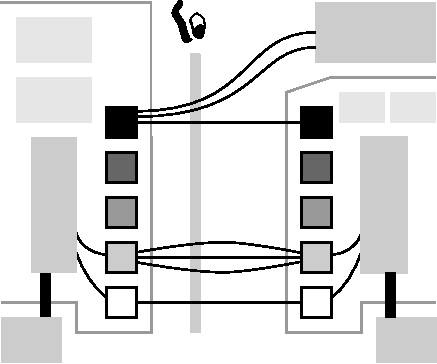
\includegraphics[width=\unitlength]{figures/arch}}%
    \put(0.475,0.7940151){\makebox(0,0)[lb]{\smash{Censor}}}%
    \put(0.1311603,0.36418277){\rotatebox{90}{\makebox(0,0)[b]{\smash{Chopper}}}}%
    \put(0.88688549,0.36418277){\rotatebox{90}{\makebox(0,0)[b]{\smash{Chopper}}}}%
    \put(0.82835114,0.58079374){\makebox(0,0)[b]{\smash{ct db}}}%
    \put(0.94671753,0.58079374){\makebox(0,0)[b]{\smash{pol en}}}%
    \put(0.28572519,0.70005326){\rotatebox{90}{\makebox(0,0)[b]{\smash{$\left.\rule{0pt}{11pt}\right\}\genfrac{}{}{0pt}{1}{\text{\fontsize{6pt}{6pt}\selectfont  Steganography}}{\text{\fontsize{6pt}{6pt}\selectfont modules}}$}}}}%
    \put(0.12359303,0.74901908){\makebox(0,0)[b]{\smash{Covertext}}}%
    \put(0.12409708,0.7156218){\makebox(0,0)[b]{\smash{Database}}}%
    \put(0.1241832,0.6146822){\makebox(0,0)[b]{\smash{Policy}}}%
    \put(0.12415816,0.58128695){\makebox(0,0)[b]{\smash{Engine}}}%
    \put(0.07224403,0.06220869){\makebox(0,0)[b]{\smash{Tor}}}%
    \put(0.07211212,0.02881384){\makebox(0,0)[b]{\smash{client}}}%
    \put(0.93102264,0.06227036){\makebox(0,0)[b]{\smash{Tor}}}%
    \put(0.93050355,0.02887435){\makebox(0,0)[b]{\smash{server}}}%
    \put(0.74234615,0.0338252){\makebox(0,0)[b]{\smash{StegoTorus}}}%
    \put(0.74157229,0.0004275){\makebox(0,0)[b]{\smash{server}}}%
    \put(0.26143011,0.03382518){\makebox(0,0)[b]{\smash{StegoTorus}}}%
    \put(0.2610434,0.0004273){\makebox(0,0)[b]{\smash{client}}}%
    \put(0.86109423,0.76926279){\makebox(0,0)[b]{\smash{Uncensored sites}}}%
    \put(0.86070205,0.73586663){\makebox(0,0)[b]{\smash{(decoy traffic)}}}%
  \end{picture}%
\endgroup%

\section{Chopping and reassembly}\label{s:chop}

\begin{figure*}[t!]%
\definecolor{hair}{gray}{1}%
\definecolor{head}{rgb}{.85,.85,1}%
\definecolor{body}{rgb}{.5,.8,.5}%
\definecolor{tail}{rgb}{.55,.55,.55}%
\centering
\begin{subfigure}[t]{.475\linewidth}
\centering
\begin{tikzpicture}[x=1.75pt,y=3ex]
\small
{\tiny
\foreach \x/\l in {0/0, 8/1, 16/2, 24/3, 32/4, 40/5, 48/6, 56/7,
                   64/8, 72/9, 80/10, 88/11, 96/12, 104/13, 112/14,
                   120/15, 128/16}
  \node [above] at (\x,0.1) {\l} ;
}
\filldraw [fill=head] (0,0) rectangle (128,-1) ;
\draw (32,0) -- (32,-1)
      (48,0) -- (48,-1)
      (64,0) -- (64,-1)
      (72,0) -- (72,-1) ;
\draw [dotted] (24, 0) -- (24, -1) ;
\node [anchor=mid,inner sep=0pt, outer sep=0pt] at (12,  -0.5) {seq no} ;
\node [anchor=mid,inner sep=0pt, outer sep=0pt] at (40,  -0.5) {$d$} ;
\node [anchor=mid,inner sep=0pt, outer sep=0pt] at (56,  -0.5) {$p$} ;
\node [anchor=mid,inner sep=0pt, outer sep=0pt] at (68,  -0.5) {$F$} ;
\node [anchor=mid,inner sep=0pt, outer sep=0pt] at (100, -0.5)
   {$\mbox{check} = 0$} ;
\filldraw [fill=body,decoration={zigzag,segment length=2ex}]
  (128,-1) decorate { -- (128,-4) } -- (0,-4) decorate { -- (0,-1) } -- cycle;
\node [anchor=mid,inner sep=0pt, outer sep=0pt] at (64,-2.5)
  {data and padding} ;
\filldraw [fill=tail] (0,-4) rectangle (128,-5) ;
\node [anchor=mid,inner sep=0pt, outer sep=0pt] at (64,-4.5)
  {authentication tag} ;
\end{tikzpicture}%
\caption{Blocks consist of a header, up to $2^{15}-1$ bytes each of
  data and padding, and an authentication tag. $d$:~data length;
  $p$:~padding length; $F$:~function code.  $d+p$ is not required to
  be a multiple of 16.\label{f:block}}
\end{subfigure}
\quad
\begin{subfigure}[t]{.47\linewidth}
\centering
\begin{tikzpicture}[x=1.75pt,y=3ex]
\small
{\tiny
\foreach \x/\l in {0/0, 8/1, 16/2, 24/3, 32/4, 40/5, 48/6, 56/7,
                   64/8, 72/9, 80/10, 88/11, 96/12, 104/13, 112/14,
                   120/15, 128/16}
  \node [above] at (\x,2.1) {\l} ;
}
\filldraw [fill=hair] (0,1) -- (0,0) -- (128,0) -- (128,2)
                            -- (88,2) -- (88,1) -- cycle;
\draw (88,1) -- (92,1) -- (92,2) ;
\node [rotate=-90] at (90,  1.5) {\tiny pad};
\node [anchor=mid,inner sep=0pt, outer sep=0pt] at (64,0.5)
 {temporary key material};
\filldraw [fill=head] (0,0) rectangle (128,-1) ;
\draw (32,0) -- (32,-1)
      (48,0) -- (48,-1)
      (64,0) -- (64,-1)
      (72,0) -- (72,-1) ;
\draw [dotted] (124,0) -- (124,-1) ;
\node [anchor=mid,inner sep=0pt, outer sep=0pt] at (16,  -0.5) {0} ;
\node [anchor=mid,inner sep=0pt, outer sep=0pt] at (40,  -0.5) {$d\!\ge\!32$} ;
\node [anchor=mid,inner sep=0pt, outer sep=0pt] at (56,  -0.5) {$p$} ;
\node [anchor=mid,inner sep=0pt, outer sep=0pt] at (68,  -0.5)
  {\footnotesize\scshape nc} ;
\node [anchor=mid,inner sep=0pt, outer sep=0pt] at (100, -0.5) {0} ;
\node [rotate=-90] at (126, -0.5) {\tiny pad};
\filldraw [fill=body,decoration={zigzag,segment length=2.1ex}]
    (0,-1) -- (128,-1) -- (128,-3) decorate { -- (128,-4) }
    -- (0,-4) decorate { -- (0,-3) } -- cycle;
\node [anchor=mid,inner sep=0pt, outer sep=0pt]
  at (64,-2) {ECDH message 1};
\node [anchor=mid,inner sep=0pt, outer sep=0pt]
  at (64,-3.5) {optional access token};
\draw (0,-3) -- (128,-3) ;
\filldraw [fill=tail] (0,-4) rectangle (128,-5) ;
\node at (64,-4.5) {authentication tag} ;
\end{tikzpicture}
\caption{A new-link request consists of a Möller key encapsulation,
  followed by a block encrypted with the temporary key material.  Four
  padding bits are copied into the “check” field to make them
  non-malleable.\label{f:cnewlink}}
\end{subfigure}
\quad
\begin{subfigure}[t]{.47\linewidth}
\centering
\begin{tikzpicture}[x=1.75pt,y=3ex]
\small
{\tiny
\foreach \x/\l in {0/0, 8/1, 16/2, 24/3, 32/4, 40/5, 48/6, 56/7,
                   64/8, 72/9, 80/10, 88/11, 96/12, 104/13, 112/14,
                   120/15, 128/16}
  \node [above] at (\x,0.1) {\l} ;
}
\filldraw [fill=head] (0,0) rectangle (128,-1) ;
\draw (32,0) -- (32,-1)
      (48,0) -- (48,-1)
      (64,0) -- (64,-1)
      (72,0) -- (72,-1) ;
\node [anchor=mid,inner sep=0pt, outer sep=0pt] at (16,  -0.5) {0} ;
\node [anchor=mid,inner sep=0pt, outer sep=0pt] at (40,  -0.5) {$d\!=\!40$} ;
\node [anchor=mid,inner sep=0pt, outer sep=0pt] at (56,  -0.5) {$p$} ;
\node [anchor=mid,inner sep=0pt, outer sep=0pt] at (68,  -0.5)
  {\footnotesize\scshape ns} ;
\node [anchor=mid,inner sep=0pt, outer sep=0pt] at (100, -0.5) {0} ;
\fill [fill=body] (0,-1) -- (128,-1) -- (128,-3) -- (32,-3) -- (32,-4)
               -- (0,-4) -- cycle;
\fill [fill=tail] (32,-3) rectangle (128,-4) (0,-4) rectangle (32,-5) ;
\draw (0,-1) rectangle (128,-3)
      (0,-3) rectangle (128,-4)
      (0,-4) -- (0,-5) -- (32,-5) -- (32,-3) ;
\node [anchor=mid,inner sep=0pt, outer sep=0pt] at (64,-2)
  {ECDH message 2};
\node [anchor=mid,inner sep=0pt, outer sep=0pt] at (16,-3.5) {new link ID};
\node [anchor=mid,inner sep=0pt, outer sep=0pt] at (80,-3.5)
  {authentication tag} ;
\end{tikzpicture}
\caption{A new-link response is a normal block, encrypted with the
  temporary key material.\label{f:snewlink}}
\end{subfigure}
\quad
\begin{subfigure}[t]{.475\linewidth}
\centering
\begin{tikzpicture}[x=1.75pt,y=3ex]
\small
{\tiny
\foreach \x/\l in {0/0, 8/1, 16/2, 24/3, 32/4, 40/5, 48/6, 56/7,
                   64/8, 72/9, 80/10, 88/11, 96/12, 104/13, 112/14,
                   120/15, 128/16}
  \node [above] at (\x,2.1) {\l} ;
}
\filldraw [fill=hair] (0,1) -- (0,0) -- (128,0) -- (128,2)
                            -- (88,2) -- (88,1) -- cycle;
\draw (88,1) -- (92,1) -- (92,2) ;
\node [rotate=-90] at (90,  1.5) {\tiny pad};
\node [anchor=mid,inner sep=0pt, outer sep=0pt] at (64,0.5)
 {temporary key material};
\filldraw [fill=head] (0,0) rectangle (128,-1) ;
\draw (32,0) -- (32,-1)
      (48,0) -- (48,-1)
      (64,0) -- (64,-1)
      (72,0) -- (72,-1) ;
\draw [dotted] (124,0) -- (124,-1) ;
\node [anchor=mid,inner sep=0pt, outer sep=0pt] at (16,  -0.5)
  {$\mbox{link ID} \ne 0$} ;
\node [anchor=mid,inner sep=0pt, outer sep=0pt] at (40,  -0.5) {0} ;
\node [anchor=mid,inner sep=0pt, outer sep=0pt] at (56,  -0.5) {0} ;
\node [anchor=mid,inner sep=0pt, outer sep=0pt] at (68,  -0.5)
  {{\footnotesize\scshape rc}} ;
\node [anchor=mid,inner sep=0pt, outer sep=0pt] at (100, -0.5) {0} ;
\node [rotate=-90] at (126, -0.5) {\tiny pad};
\end{tikzpicture}%
\caption{A reconnection request is just a key encapsulation and a
  modified header. The link ID replaces the sequence number, $d$ and
  $p$ must be zero, and there is no authentication tag.\label{f:creconn}}
\end{subfigure}
\caption{Message formats before steganography.  Background shading
  indicates encryption mode.  {\color{head}$\blacksquare$}:~header
  encryption; {\color{body}$\blacksquare$}:~GCM encryption;
  {\color{tail}$\blacksquare$}:~GCM authentication tag;
  {$\square$}:~Möller key encapsulation.  There are 16 bytes per row
  of each diagram.\label{f:msgfmt}}
\end{figure*}


As we described briefly in Section~\ref{s:arch}, chopping converts the
traffic on a Tor link into a more malleable format: a sequence of
variable-size \emph{blocks}, independently padded and deliverable out
of order.  Every byte of each block is computationally
indistinguishable from randomness, as defined in~\cite{s-noncephil};
this is a baseline requirement for the hiddentext in theoretically
secure steganographic schemes.~\cite{s-ah-pssteg,s-ah-pksteg}  The
module that performs this job (and its inverse) is, naturally, called
the \emph{chopper}.

The block format is shown in Figure~\ref{f:block}.  The bulk of each
block is encrypted using AES in GCM mode~\cite{s-gcm}, which provides
both confidentiality and message integrity~\cite{s-authenc}.  The
block header consists of a 32-bit sequence number; two length fields,
$d$ and $p$, indicating respectively how much data and padding the
block carries; an opcode field, $F$, discussed below; and a 56-bit
check field, which must be zero.  The minimum block length is $32$
bytes ($128$-bit header, $128$-bit MAC) and the maximum is $2^{17} +
32$ bytes.  Block length is controlled by the steganography modules;
the chopper will fabricate blocks exactly as long as requested, using
data if possible, padding if there is not enough.  Padding consists of
binary zeroes.  Blocks containing only padding ($d=0$) are generated
when there is no data available but the cover protocol requires
transmission.

The sequence number permits the receiver to sort incoming blocks into
their original order.  It serves the same function as a TCP sequence
number, but it always starts at zero, counts blocks rather than bytes,
and may not wrap around (see Section~\ref{s:rekey}).  It also serves
to ensure that the same header is never transmitted twice.  This is
important because the header must also be encrypted to render it
indistinguishable from randomness, and needs integrity protection to
preclude chosen-ciphertext attacks~\cite{a-padding-oracle,a-ssh-plaintext},
but we can't include it in the data authenticated by GCM because we
have to decrypt $d$ and $p$ in order to know where the authentication
tag begins.

Instead, we protect the header with a custom short-message
authenticated encryption mode that relies only on the basic AES
pseudorandom permutation.  The check field brings the header up to
exactly the AES block size, and we encrypt it as a standalone block
with a different key from that used for the payload.  Before the
receiver acts on a decrypted header, it verifies that every bit of the
check field is zero, and that the sequence number is within a
256-block-wide receive window.  An active attacker who modifies the
ciphertext of the header has less than one chance in $2^{80}$ of
passing this verification.  We recycle the \emph{ciphertext} of the
header as the GCM nonce for the payload.

\subsection{Function Codes}\label{s:f-codes}

The $F$ field of the block header controls how the receiver will
process the block. All presently-defined codes are listed in
Table~\ref{t:fcodes}.  Some codes are only valid in handshakes; see
below.

\begin{table}[h!]
\begin{tabular}{rlp{.70\columnwidth}}
\toprule
\textbf{No.} & \textbf{Name} & \textbf{Semantics} \\
\midrule
0   & \textsc{data} & Application data to be relayed.\\
1   & \textsc{fin}  & Last block of application data to be relayed.\\
2   & \textsc{rst}  & Protocol error; close the link immediately.\\
3   & \textsc{rc}   & Reconnect: associate this new connection with an
                      existing link.\\
4   & \textsc{nc}   & New link, client side.
                      See section~\ref{s:handshake} for details.\\
5   & \textsc{ns}   & New link, server side.\\
6   & \textsc{rki}  & Initiate rekeying; see
                      Section~\ref{s:rekey} for details.\\
7   & \textsc{rkr}  & Respond to rekeying.\\
8\rlap{--127}&      & Reserved for future definition.\\
128\rlap{--255}&    & Reserved for steganography modules.\\
\bottomrule
\end{tabular}
\caption{Codes for the $F$ field}\label{t:fcodes}
\end{table}

\subsection{Handshake Messages}\label{s:handshake}

The first few bytes of data sent on each new connection are a
\emph{handshake message} (henceforth just “handshake”), which informs
the server whether this connection belongs to an existing link or to a
new one.  If the connection belongs to a new link, the server replies
with a handshake of its own, and both peers derive new session keys
for the link from the data in the handshakes.  There are three
handshake formats, shown in figures~\ref{f:cnewlink}, \ref{f:creconn},
and~\ref{f:snewlink}.  Handshakes have similar overall structure to
blocks, but vary in details.

Most asymmetric cryptosystems' ciphertexts are easily distinguished
from randomness. We use Möller's elliptic-curve key encapsulation
mechanism~\cite{s-moller}, which is designed to produce random
ciphertexts. It can only be used to establish a weak shared secret,
which we refer to as “temporary key material.”  It has the unfortunate
property of producing 164-\emph{bit} messages, which must be padded to
a whole number of bytes.  The padding bits could be flipped by an
adversary without any visible effect.  To prevent this information
leak, the \emph{check} field of the header that immediately follows a
key encapsulation contains a copy of the padding.  Also, the server
must maintain a replay cache of all key encapsulations it has seen
recently, and discard any handshake with a replayed encapsulation,
even if the data that follows is different.

Each link has a nonzero, 32-bit \emph{link ID}.  The server chooses
this ID during link setup, making sure that it is unique among all
active or recently-active connections to the same server.  It is never
transmitted in cleartext, so it need not be random.

Key derivation, whether from the temporary key material or from
Diffie-Hellman exchanges, is done with HKDF-SHA256~\cite{s-hkdf1},
salted with the server's public key, and produces four 128-bit AES
keys: server-to-client payload key, server-to-client header key,
client-to-server payload key, and client-to-server header key, in that
order.

\subsubsection{New Link Handshake}

Link setup is loosely based on the STS protocol~\cite{s-sts} and
provides forward secrecy.  Initially, the client knows the server's
public key.  It has no asymmetric keypair of its own, but it may have
an “access token” which will identify it to the server.  This token is
opaque to the client, and its contents are outside the scope of this
paper.

The client's first message to the server is shown in
figure~\ref{f:cnewlink}.  It begins with a randomly chosen Möller key
encapsulation, followed by a special block encrypted with the
temporary key material.  This block has sequence number 0, and its $F$
code is \textsc{rc}.  Its first 32 bytes are an ECDH message on the
NIST standard curve P-256~\cite{s-fips186-2}, derived from a source of
strong randomness.  Only the $x$-coordinate of the public point is
transmitted.  If the client has an access token, it follows
immediately after the ECDH message.

If the server can decrypt this handshake and finds the access token
(if any) acceptable, it replies with its own handshake, shown in
figure~\ref{f:snewlink}.  This is a normal block, also encrypted with
the temporary key material provided by the client.  It also has
sequence number 0, its $F$ code is \textsc{rs}, and its contents are
another ECDH message and the link ID for the new link.  Once the
client receives this message, both sides can complete the
Diffie-Hellman exchange and derive long-lived keys for the link.
Subsequent blocks are encrypted with those keys.  The handshakes count
as sequence number 0 in each direction.

\subsubsection{Reconnection Handshake}

For new connections to established links, the client's handshake needs
to be as short as possible.  It is shown in figure~\ref{f:creconn}.
As with a new-link handshake, it begins with a randomly chosen Möller
key encapsulation, but instead of a block, only a modified header
follows.  This header has $p=0$, $d=0$, and $F=\text{\textsc{rc}}$,
and it carries the desired link ID in place of the sequence number.
Unlike normal blocks with $p=0$ and $d=0$, the GCM authentication tag
is omitted.  The client may transmit blocks, encrypted with the
appropriate link keys, immediately after this handshake (that is, in
the same cover-protocol message).

\subsection{Rekeying}\label{s:rekey}

Rekeying is very similar to key derivation for a new link, but uses
blocks rather than special handshake messages.  Rekeying resets the
sequence number but does not change the link ID.  Either peer may
initiate a rekeying cycle at any time by transmitting an
\textsc{rki} block.  Peers are \emph{required} to rekey before the
sequence number wraps around, and encouraged to rekey considerably
sooner.

An \textsc{rki} block's data section is simply an ECDH message on curve
P-256.  The recipient of this message responds with an \textsc{rkr}
block, whose data section is another ECDH message.  Upon receipt of
\textsc{rkr}, both peers derive new link keys from the Diffie-Hellman
exchange, just as they would have for a new link.  It is a protocol
error to transmit any blocks after \textsc{rki} until receipt of
\textsc{rkr}, or to transmit blocks using the old keys after
transmitting \textsc{rkr}.

\subsection{Link Termination}

When both sides have sent and received a \textsc{fin} block, the link
is closed; however, both sides must remember the link ID for some
time, to guard against replay attacks or delayed block arrival.  It is
a protocol error to transmit a \textsc{data} block with a nonzero $d$
field after transmitting a \textsc{fin} block; however, \textsc{data}
blocks with $d=0$ may still be sent, and other function codes may be
used if appropriate.  For instance, the \textsc{rki} block requires a
response, even if the recipient has already transmitted a
\textsc{fin}.

\section{Steganography}\label{s:steg}

In this section, we describe two proof-of-concept steganography
modules: one that duplicates the packet sizes and timings of encrypted
peer-to-peer protocols, and one that mimics HTTP.  These modules
illustrate the flexibility and feasibility of the StegoTorus
framework.  However, they are not expected to resist sophisticated,
targeted attacks that might be launched by a nation-state adversary.
To underscore this, for each module we also describe potential attacks
and the level of sophistication each requires.

More diverse and resilient modules are under development, both by us
and the larger community, as the arms race continues.  The StegoTorus
client can be configured to use whichever modules the adversary has
not yet blocked; therefore, ultimately, the adversary will have to
detect and block traffic generated by \emph{all} of the steganography
modules in order to block StegoTorus.

\subsection{Embed Module}

The \emph{embed} steganography module conceals Tor traffic within an
encrypted, peer-to-peer cover protocol, such as the popular Skype and
Ventrilo protocols for secure voice over IP.  (Ventrilo is not
strictly a peer-to-peer protocol, but its users typically set up their
own servers, so there is no small, stable set of server IPs that could
be whitelisted.)  Since the audio payload of each packet is encrypted,
we can substitute our own encrypted data without fear of payload
inspection.  This leaves cleartext headers, packet sizes, and
inter-packet timings as the characteristics visible to the censor.

\subsubsection{Packet Traces}

This module relies on a database of \emph{packet traces}, pre-recorded
sequences of packet sizes and timings from real sessions of the cover
protocol.  Client and server match the recorded packet sizes exactly,
and timings to the nearest millisecond.  If there is no data available
when a packet should be sent, they will fabricate padding-only blocks
to maintain the deception.

The server does not maintain its own database of traces; instead, the
client transmits its chosen trace to the server as a special control
message, immediately after link setup.  Some of these traces are
distributed with the software, but users are encouraged to capture
their own use of the cover protocol, so that the censor cannot block
StegoTorus by pattern-matching against the distributed set of traces.
(Packet timings seen by the client may or may not correspond to packet
timings as actually transmitted by the server.  For greater realism,
one should capture a trace from both ends, but we have not implemented
this yet.)

\smallskip\noindent\textbf{Potential Attacks:} Some VoIP protocols
permit an eavesdropping adversary to learn much about the speech being
transmitted, just from packet sizes and timings~\cite{a-foniks}.
Therefore, if traces are reused too often, the censor might become
suspicious of users apparently having the exact same conversation over
and over again.

\subsubsection{Application Headers}

The packet trace does not attempt to capture application headers, as
these may depend on the substituted contents.  Instead, the
\emph{embed} module includes emulation code for each potential cover
protocol.  Unfortunately, neither the Skype nor the Ventrilo protocol
has a public specification, necessitating reverse engineering.  To
date this has been done by hand, but we are investigating the
possibility of automating the
process~\cite{a-polyglot,a-discoverer,a-ctxtaware}.

\smallskip\noindent\textbf{Potential Attacks:} If the censor has
access to the true protocol specification for a protocol we have
reverse engineered, they may be able to detect deviations on our
part.

Even if the censor doesn't have this information, it might choose to
block \emph{all} apparent VoIP protocols, or all peer-to-peer traffic
that appears to contain encrypted data.  These are popular, but not
yet so popular that this would amount to “turning off the Internet,”
and there are plausible political cover stories for such actions by a
nation-state: preserving telephone revenue, combating copyright
infringement, etc.

\subsection{HTTP Module}

The \emph{HTTP} steganography module simulates unencrypted HTTP
traffic.  Since the censor can observe the overt content of this
module's traffic, and protocol decoders for HTTP are ubiquitous, we
take care to mimic “real” browser and website behavior as accurately
as possible.

HTTP~\cite{s-http} follows a strict pattern: the client sends a
\emph{request}, waits for the server to produce a \emph{response}, can
then send another request, and so on.  HTTP~1.1 allows the client to
send several requests in a row without waiting for responses
(“pipelining”) but this is rarely used, due to server
bugs~\cite{s-pipeline}.  Instead, clients achieve parallelism by
opening multiple connections to the same server.  Each request
contains a “method” (\textsc{get}, \textsc{post}, etc) that controls
what the server will do to prepare the response.

The \emph{HTTP} module also relies on a database of pre-recorded HTTP
requests and responses; we also refer to these as “traces.”  Like the
\emph{embed} module's traces, some are distributed with the program,
and users are encouraged to record their own.  Unlike \emph{embed},
requests and responses are not organized into a temporal sequence, and
client and server use independent databases.  However, the server
generates responses that are consistent with client requests; for
instance, if a client sends a request for a PDF document, the server
will produce a PDF covertext.

\subsubsection{Request Generator}

Normal HTTP client-to-server traffic consists almost entirely of
\textsc{get} requests.  Unfortunately, these provide very little space
to conceal our hiddentexts.  Here is a typical request template from
our database:

\begin{lstlisting}
GET /<uri> HTTP/1.1
Accept: text/html,application/xhtml+xml,
    application/xml;q=0.9,*/*;q=0.8
Accept-Encoding: gzip, deflate
Accept-Language: en-us,en;q=0.5
Connection: keep-alive
Host: <host>
User-Agent: Mozilla/5.0 (X11; Linux x86_64; rv:10.0)
    Gecko/20100101 Firefox/10.0
Cookie: <cookie>
\end{lstlisting}

\noindent Nearly all of this is boilerplate that must be sent verbatim
in every request.  Data can be inserted at each position marked
\textitt{<\ldots>}, but it must be properly encoded.

At present we only store hiddentext in the \textitt{<uri>} and
\textitt{<cookie>} positions, which can carry arbitrary textual data.
We encode the binary chopper output in a modified \texttt{base64}
alphabet~\cite{s-base64} that avoids characters with special meaning
in URIs or cookies: `\texttt{+}' is replaced by `\texttt{-}',
`\texttt{/}' by `\texttt{\_}', and `\texttt{=}' by `\texttt{.}'.  We
then insert characters at random positions in the encoded string, to
make it look more like a genuine URI or cookie header: for URIs we
insert `\texttt{/}', for cookies we alternate between `\texttt{=}' and
`\texttt{;}'.

The \textitt{<host>} can theoretically also carry hiddentext, but with
more difficulty: \textitt{<host>} must have the form of a DNS hostname
or IP address~\cite{s-http}, and the censor could block HTTP
connections where it was not a registered hostname for the IP address
to which the client was connected.  Presently, we do not attempt this;
instead we do a reverse DNS lookup on the server's IP address, and use
the first reported name in every request to that address.

\smallskip\noindent\textbf{Potential Attacks:}
To the human eye, the HTTP request generator's URIs and cookies likely
look different from normal URIs or cookies.  The pattern of requests
that it generates is also potentially different from the pattern of
requests generated by a visit to a real website.  Hence, it would be
possible for an adversary to build a machine classifier that can make
the same judgment.  The cookie string we send changes on every
request, without the server sending back \texttt{Set-Cookie:}
directives; this could also be a distinguisher, as a real web browser
only changes cookies when instructed to.  If such attacks become
common, they we may be limited in our use of cookies as a carrier
channel.  More sophisticated cookie, URI, and request pattern
generation is also possible; Infranet~\cite{c-infranet}, for instance,
devotes some effort to this problem.  However, substantially more
overhead will be required.

The \texttt{User-Agent} header identifies the browser and operating
system in use.  If the same client IP address consistently produces
one user-agent, except during a handful of browsing sessions, that
handful might attract attention.  Generating a database of client
requests on each user's machine ensures that we generate user-agent
headers matching the browser that that user normally uses.

The censor may conduct active attacks by replaying HTTP requests; a
real web server would normally produce the same response, but
StegoTorus will not.  To mitigate this we could place an off-the-shelf
HTTP “accelerator” cache in front of the StegoTorus server so that,
for a short time, replayed requests would produce the same response as
the original.

\subsubsection{Response Generator}

HTTP responses begin with a few headers, similar to the ones shown
above, but offering even less space for hiddentext.  However, they
continue with a “response body” which is \emph{designed} to carry
arbitrary data.  That data typically conforms to some known file
format, which must be consistent with the contents of the request.  We
have developed response generators that embed StegoTorus hiddentexts
in three common file formats: JavaScript, PDF, and Flash.  These data
formats are complex enough to conceal hiddentexts easily, and
pervasive enough that blocking them would break far too many popular
websites to be politically tenable.  Generators for HTML and various
image, audio, and video formats are under development.

\smallskip\noindent\textbf{JavaScript Generator:} JavaScript is a
programming language, human-readable in its original form, but
frequently “minified” to reduce its size on the wire. Minification
involves removing all white space and replacing variable names with
shorter machine-generated identifiers.  There is an enormous volume of
JavaScript in use on the open web: 2.5\% of all bytes transferred by
HTTP in early 2009~\cite{a-res-traffic}.

This generator picks a response containing JavaScript, scans it for
identifiers and numbers, and replaces them with characters from the
hexadecimal encoding of the hiddentext.  To preserve syntactic validity,
the encoder will not change the first character of an identifier or a
number, and there is a blacklist of JavaScript keywords and built-in
functions that should not be replaced.  The decoder simply reverses
the process.  Our objective with this module is to produce syntactically
valid JavaScript that cannot be trivially detected by a parser.

\smallskip\noindent\textbf{PDF Generator:} PDF documents consist of a
sequence of “objects,” which define pages, images, fonts, and so on.
Many of these objects will normally be compressed, using the
ubiquitous “deflate” algorithm, to save space.  The PDF response
generator locates compressed objects within a PDF document from the
HTTP response database, and replaces their contents with our
hiddentexts.  Chopper output is incompressible, but we apply the
“deflate” transformation to it anyway, so that each modified object's
contents is still superficially what it ought to be.  The overall file
structure is adjusted to match.

\smallskip\noindent\textbf{SWF Generator:} Adobe (formerly Shockwave)
Flash is a format for vector-graphic animations, and is also
frequently used as a container for video.  Flash files consist of a
sequence of tagged data blocks, containing shapes, buttons, bitmaps,
ActionScript byte code, etc.~\cite{s-flash} Flash files may be
compressed (CWS) or uncompressed (FWS). In the more common CWS format,
the entire file (with the exception of a short initial header, but
including the block framing) is compressed with “deflate.”  The SWF
response generator uncompresses a template CWS file, replaces block
contents with encrypted data, and recompresses the result.

\smallskip\noindent\textbf{Potential Attacks:}
The HTTP response generator attempts to preserve the syntactic
validity of JavaScript, PDF and SWF files that it modifies.  However,
it does not attempt to preserve the semantics of JavaScript or the
original content of PDF or SWF.  Therefore, adversaries might be able
to detect the use of the present HTTP generator by attempting to
execute JavaScript, render PDF documents, or play back Flash
animations.  However, doing so at line rate on a border router would
be quite challenging.  The filter would have to extract HTTP response
bodies of interest, reassemble packets into streams, and then parse
and decode the contents of the file; all of these are expensive and
complicated operations.  Providing the appropriate execution
environment for JavaScript requires the adversary to assemble and
process all the data of the surrounding webpage, just as a browser
would.

Nonetheless, we do expect that if StegoTorus comes into wide use,
filtering routers will gain the ability to detect these simple
schemes.  In particular, a natural escalation of the arms race might
involve the use of cascading detectors, where a series of fast filters
select traffic to subject to more expensive analyses.  If this
happens, we would have to implement more sophisticated steganography.


\begin{figure*}[t!]
\centering
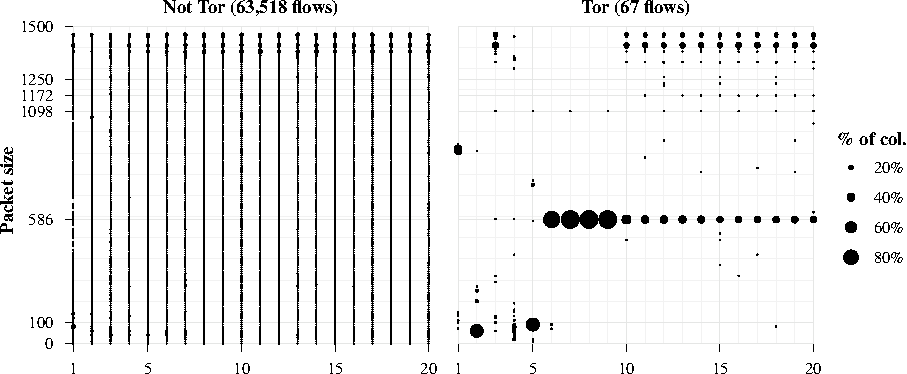
\includegraphics{figures/https-patterns-c}
\caption{Payload lengths for the first 20 non-empty packets of 63,585
  unidirectional flows on TCP port 443, taken from the CAIDA
  2011-Chicago data set.~\cite{d-caida} Port 443 is officially assigned
  to HTTP over TLS, but Tor relays are sometimes configured to accept
  connections on this port. Scanning for 586-byte TCP payloads
  identifies 67~of the flows as probable Tor traffic.}\label{f:packetlengths}
\end{figure*}

\begin{figure*}[t!]
\centering
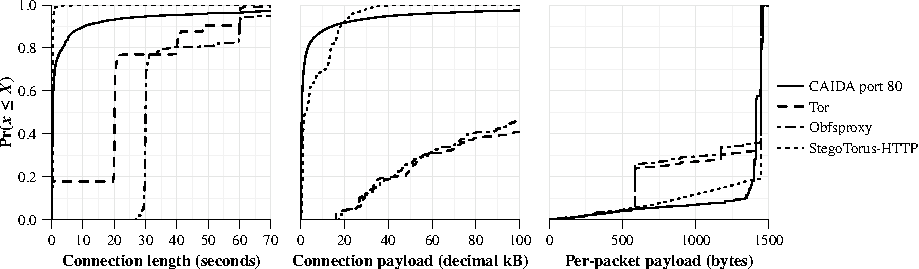
\includegraphics{plots/ecdf-cl-bw-pl}
\caption{Empirical CDFs of connection length, total data transferred,
  and per-packet payload for 20 visits to each of the Alexa top ten
  websites, using Tor directly (dashed line), obfsproxy (dot-dash
  line), and StegoTorus-HTTP (dotted line).  CAIDA Chicago-2011 port
  80 traffic for reference (solid line).} \label{fig:ECDFs}
\end{figure*}

\section{Detection Resistance}\label{s:attacks}

To evaluate how well StegoTorus can conceal a Tor stream, we developed
two attacks upon Tor, which StegoTorus ought to defeat if it is
functioning as intended.  We designed these attacks to be practical in
the resource-constrained environment of a perimeter filter (as
described in Section~\ref{s:limits-censor}) so they are deliberately
quite simple.  The first attack picks Tor streams out of other TCP
streams, based on a fundamental characteristic of the Tor wire
protocol that is cheap to detect.  The second attack operates on known
Tor streams and extracts information about the sites being visited
covertly.  In each case we will first describe the attack and how it
fares against Tor, then discuss its effectiveness against StegoTorus.
As we did for the steganography modules, we will also discuss
potential improvements to the attacks that might be implemented by an
adversary determined to detect StegoTorus.

\subsection{Detecting Tor}\label{s:detect-tor}

The Tor protocol~\cite{s-tor} sends nearly all messages in the form of
“cells” with a fixed length of 512 bytes.  These cells are packed into
TLS~1.0 application-data records~\cite{s-tls1} on the wire.  Because
of the “empty record” countermeasure for a cryptographic weakness in
TLS 1.0~\cite{a-ssl-cp1,a-ssl-cp2}, the overhead of TLS encapsulation
is 74 bytes per application-data record.  The client will pack many
cells into a record if it has enough to say, and TCP will split large
records in the middle in order to transmit MTU-sized packets, but Tor
nonetheless winds up transmitting many TCP packets that contain
exactly one cell.  These packets have a characteristic payload length
of 586 bytes.  A filtering router can pick Tor streams out of other
traffic by counting how often they appear.

We implemented the following concrete algorithm: let $\tau$ be the
adversary's current estimate of the probability that a given TCP flow
is Tor, initially set to zero.  Ignore packets containing only an ACK
and no payload; these are best treated as neutral~\cite{a-finger-onion}.
Otherwise, update
\(
\tau \leftarrow \alpha \tau + (1 - \alpha) \mathbf{1}_{l=586}
\)
where $\alpha \in (0,1)$ is a tuning parameter and
$\mathbf{1}_{l=586}$ is one if the TCP payload length $l$ equals 586
bytes, zero otherwise.  If $\tau$ rises past a threshold value $T$,
the TCP flow is considered Tor traffic.

To do this, a perimeter filter must be capable of tracking TCP flows
in realtime, and maintaining one scalar value (the estimate $\tau$)
for each; to the best of our knowledge, this is within the
capabilities of modern DPI hardware.  Empirically, $\alpha = 0.1$ and
$T = 0.4$ identifies Tor within a few dozen packets.
Figure~\ref{f:packetlengths} shows probable Tor flows picked out of
all the port-443 traffic in the CAIDA 2011-Chicago
data set~\cite{d-caida} with this technique.  (This data set only
includes IP and TCP headers for each packet captured, so we are unable
to confirm that the selected flows are actually Tor, or how much of
the background traffic is in fact HTTPS.)

To confirm the effectiveness of this attack against vanilla Tor, we
collected traffic traces from visiting the top ten Alexa sites twenty
times over vanilla Tor, obfsproxy~\cite{n-iran-ob}, and StegoTorus
with the \textit{HTTP} steganography module.  In addition to non-zero
TCP payload sizes for each packet, we extracted the lifetime and total
data transferred (treating the two directions as independent) of each
TCP stream.  Figure~\ref{fig:ECDFs} presents a qualitative comparison
of these features in the form of empirical CDFs, with all TCP flows on
port 80 of the CAIDA 2011-Chicago data set (again, we cannot confirm
this, but port 80 traffic on the public Internet is almost surely
HTTP) for reference.  Tor's predilection for generating 586-byte
packets is clearly seen in the rightmost panel of
Figure~\ref{fig:ECDFs}, and the other panels show other
characteristics that would be easy for the adversary to detect, such
as a tendency for TCP connections to last exactly 20 or 30 seconds.
Obfsproxy does little to alter these features.

StegoTorus fares much better.  It is not perfect, but it generates
empirical CDFs for all three features that are closer to the CAIDA
port 80 reference than they are to either Tor or obfsproxy.  In
particular, it eliminates the 586-byte characteristic payload size.
Still, a determined adversary with more analytic power at its disposal
might be able to detect the remaining statistical differences between
StegoTorus-HTTP and “normal” HTTP traffic that Figure~\ref{fig:ECDFs}
reveals.  Improving our HTTP emulation will reduce these differences.
If necessary, we could also implement an explicit statistical model of
what HTTP traffic “should” be like.

\subsection{Identifying Visits to Facebook}\label{s:detect-fb}

Once the censor has identified TCP streams as Tor traffic, they would
also like to learn which sites are being accessed clandestinely.  We
present a simple method to determine whether a Tor user is visiting
Facebook; this site has sometimes been completely blocked by
government censors.  It is a cut-down version of Panchenko
et~al.~\cite{a-finger-onion}, which can identify accesses to a small
set of censored websites within a larger Tor session.  Their
classifier uses a support vector machine, which is too expensive to
run on a filtering router, even on a small number of streams. With
careful optimization, our classifier requires a handful of probability
calculations per arriving packet, plus maintenance of a sliding-window
vector per stream under surveillance; this should be acceptably cheap.

Once a stream has been identified as Tor traffic, the censor maintains
a pair of sequences, ${u_i}$ and ${d_i}$, sliding over the last $n$
non-empty packets observed by the filtering router.  Each $u_i$ is the
cumulative sum of payload lengths for packets $1$ through $i$ sent
“upward” (client to relay), and $d_i$ is the same for packets sent
“downward” (relay to client). The censor has previously observed
“typical” Facebook traffic, and modeled the probability distributions
$\Pr[U_i]$ and $\Pr[D_i]$ that one would expect to see if a trace were
a visit to Facebook.  Using this model, the censor computes
\begin{multline*}
\log \Pr\left[\{u_i\},\{d_i\} \text{ is Facebook}\right]\\
= \sum_{i=1}^n \log \Pr[U_i=u_i] + \sum_{i=1}^n \log \Pr[D_i=d_i]
\end{multline*}
Log-probabilities are used to avoid floating-point underflow, since
the per-packet probabilities can be very small.  If the overall
log-probability exceeds a threshold, the censor classifies the traffic
as a visit to Facebook.

\begin{figure}[h]
\centering
% Generated by fb-detect.R from fb-detect.csv, then manually edited to
% ensure that the labels for the five labeled points do not overlap,
% give those points their own style in the legend, remove all
% clipping, adjust font and line sizes finely, clean up redundant or
% unnecessary drawing operations, and eliminate all use of opacity
% (partial opacity is not needed, and merely having /CA settings in
% the PDF can cause issues downstream).
%
% Most of the above adjustments are cosmetic, but the manual tuning of
% point labels is essential.
%
% If you modify this file, take care not to introduce any uncommented
% whitespace, _including newlines_, outside the tikzpicture environment;
% it can cause things to move around in the overall document.
%
% Created by tikzDevice version 0.6.2 on 2012-01-07 21:07:33
% !TEX encoding = UTF-8 Unicode
\beginpgfgraphicnamed{figures/fb-detect-c}%
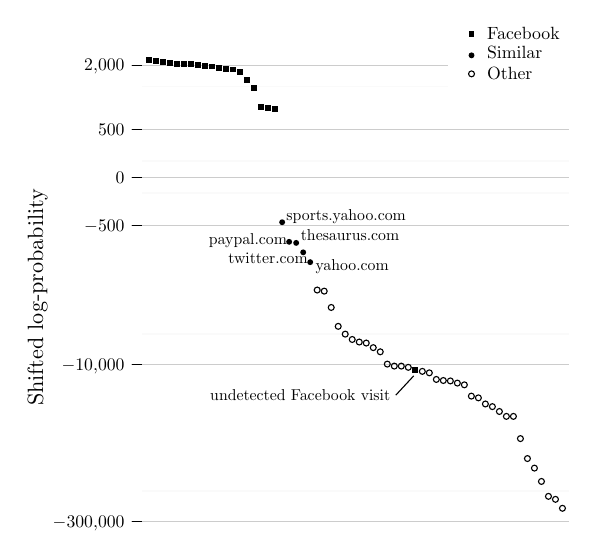
\begin{tikzpicture}[x=1pt,y=1pt]

% legend
\fill (168.31,199.48) rectangle	(170.44,201.62);
\fill (169.37,192.79) circle (  1.07);
\draw (169.37,186.10) circle (  1.07);

\begin{scope}[anchor=base west, inner sep=0pt, outer sep=0pt]
\node [scale=0.64] at (175,198.35) {Facebook};
\node [scale=0.64] at (175,191.52) {Similar};
\node [scale=0.64] at (175,183.89) {Other};
\end{scope}

% y-axis labels
\node[rotate=90,anchor=base,inner sep=0pt,outer sep=0pt,scale=0.8]
  at ( 14.54,105.39) {Shifted log-probability};

\begin{scope}[anchor=base east, inner sep=0pt, outer sep=0pt]
\node[scale=0.64] at ( 44, 22.05) {$-$300,000};
\node[scale=0.64] at ( 44, 79.06) {$-$10,000};
\node[scale=0.64] at ( 44,129.28) {$-$500};
\node[scale=0.64] at ( 44,146.60) {0};
\node[scale=0.64] at ( 44,163.93) {500};
\node[scale=0.64] at ( 44,187.17) {2,000};
\end{scope}

% y-ticks
\begin{scope}[line width=0.2pt, line cap=round]
\draw ( 46.68, 24.25) -- ( 50.30, 24.25);
\draw ( 46.68, 81.26) -- ( 50.30, 81.26);
\draw ( 46.68,131.48) -- ( 50.30,131.48);
\draw ( 46.68,148.81) -- ( 50.30,148.81);
\draw ( 46.68,166.14) -- ( 50.30,166.14);
\draw ( 46.68,189.37) -- ( 50.30,189.37);
\end{scope}

% y-grid
\definecolor[named]{gridminor}{gray}{0.98}
\definecolor[named]{gridmajor}{gray}{0.80}

\begin{scope}[color=gridminor, line width=0.6pt]
\draw ( 50.30, 35.32) -- (204.77, 35.32);
\draw ( 50.30, 92.07) -- (204.77, 92.07);
\draw ( 50.30,143.10) -- (204.77,143.10);
\draw ( 50.30,154.52) -- (204.77,154.52);
\draw ( 50.30,181.49) -- (160.77,181.49);
\end{scope}

\begin{scope}[color=gridmajor, line width=0.2pt]
\draw ( 50.30, 24.25) -- (204.77, 24.25);
\draw ( 50.30, 81.26) -- (204.77, 81.26);
\draw ( 50.30,131.48) -- (204.77,131.48);
\draw ( 50.30,148.81) -- (204.77,148.81);
\draw ( 50.30,166.14) -- (204.77,166.14);
\draw ( 50.30,189.37) -- (160.77,189.37);
\end{scope}

% data
\fill ( 51.76,189.97) rectangle ( 53.90,192.10);
\fill ( 54.29,189.73) rectangle ( 56.43,191.86);
\fill ( 56.83,189.16) rectangle ( 58.96,191.30);
\fill ( 59.36,189.00) rectangle ( 61.49,191.13);
\fill ( 61.89,188.72) rectangle ( 64.02,190.85);
\fill ( 64.42,188.60) rectangle ( 66.56,190.73);
\fill ( 66.96,188.48) rectangle ( 69.09,190.61);
\fill ( 69.49,188.27) rectangle ( 71.62,190.40);
\fill ( 72.02,187.74) rectangle ( 74.15,189.87);
\fill ( 74.55,187.71) rectangle ( 76.69,189.84);
\fill ( 77.08,187.26) rectangle ( 79.22,189.40);
\fill ( 79.62,186.66) rectangle ( 81.75,188.79);
\fill ( 82.15,186.60) rectangle ( 84.28,188.73);
\fill ( 84.68,185.71) rectangle ( 86.82,187.85);
\fill ( 87.21,182.98) rectangle ( 89.35,185.12);
\fill ( 89.75,179.87) rectangle ( 91.88,182.01);
\fill ( 92.28,173.20) rectangle ( 94.41,175.34);
\fill ( 94.81,172.65) rectangle ( 96.94,174.78);
\fill ( 97.34,172.34) rectangle ( 99.48,174.47);

\fill (147.99, 77.88) rectangle (150.12, 80.02);
\coordinate (fp) at (148.5, 77); % used below
\coordinate (fpl) at (142, 70);

\fill (100.94,132.49) circle (  1.07);
\fill (103.47,125.41) circle (  1.07);
\fill (106.01,125.02) circle (  1.07);
\fill (108.54,121.61) circle (  1.07);
\fill (111.07,118.06) circle (  1.07);

\draw (113.60,107.99) circle (  1.07);
\draw (116.14,107.59) circle (  1.07);
\draw (118.67,101.69) circle (  1.07);
\draw (121.20, 94.87) circle (  1.07);
\draw (123.73, 92.06) circle (  1.07);
\draw (126.26, 90.12) circle (  1.07);
\draw (128.80, 89.20) circle (  1.07);
\draw (131.33, 88.83) circle (  1.07);
\draw (133.86, 87.17) circle (  1.07);
\draw (136.39, 85.67) circle (  1.07);
\draw (138.93, 81.23) circle (  1.07);
\draw (141.46, 80.51) circle (  1.07);
\draw (143.99, 80.50) circle (  1.07);
\draw (146.52, 80.06) circle (  1.07);
\draw (151.59, 78.60) circle (  1.07);
\draw (154.12, 78.07) circle (  1.07);
\draw (156.65, 75.68) circle (  1.07);
\draw (159.18, 75.30) circle (  1.07);
\draw (161.72, 75.14) circle (  1.07);
\draw (164.25, 74.37) circle (  1.07);
\draw (166.78, 73.74) circle (  1.07);
\draw (169.31, 69.65) circle (  1.07);
\draw (171.85, 69.03) circle (  1.07);
\draw (174.38, 66.82) circle (  1.07);
\draw (176.91, 65.86) circle (  1.07);
\draw (179.44, 64.10) circle (  1.07);
\draw (181.97, 62.33) circle (  1.07);
\draw (184.51, 62.33) circle (  1.07);
\draw (187.04, 54.31) circle (  1.07);
\draw (189.57, 47.10) circle (  1.07);
\draw (192.10, 43.64) circle (  1.07);
\draw (194.64, 38.82) circle (  1.07);
\draw (197.17, 33.44) circle (  1.07);
\draw (199.70, 32.36) circle (  1.07);
\draw (202.23, 29.12) circle (  1.07);

% point labels
\begin{scope}[anchor=base west, inner sep=0pt, outer sep=0pt]
\node [scale=0.57] at (102.5,133) {sports.yahoo.com};
\node [scale=0.57] at (74.5,124.5) {paypal.com};
\node [scale=0.57] at (107.7,126) {thesaurus.com};
\node [scale=0.57] at (81.5,117.5) {twitter.com};
\node [scale=0.57] at (113,115) {yahoo.com};
\end{scope}

\draw (fp) -- (fpl);
\node [anchor=east, scale=0.57] at (fpl) {undetected Facebook visit};

\end{tikzpicture}\endpgfgraphicnamed%

\caption{Log-probabilities reported by Facebook classifier, shifted to
  place the classification threshold at zero on the y-axis. Visits to
  Facebook (squares) show the shifted log-probability for the first
  250 packets. Visits to non-Facebook sites (circles) show the maximum
  shifted log-probability observed for a 250-packet sliding
  window.}
\label{f:prob-facebook}
\end{figure}

We trained this classifier on the first $250$ packets transmitted in
each direction over ten visits to the Facebook home page (login
screen), and modeled the probability distributions as independent
Gaussians for each position in the sequence. This is a deliberate
departure from reality: $U_{i+1}$ has a strong dependence on $U_i$,
since they are cumulative sums, but treating them as independent makes
the classifier robust to variation in the order of resources
downloaded.  We then tested it on 20 more visits to Facebook, plus 40
visits to other web sites chosen from Alexa's categorized directory of
popular sites~\cite{d-alexa}.  For all of the test visits, we browsed
randomly until we had somewhere between 5,000 and 30,000 TCP packets;
this resulted in a total of over 450,000 total packets and 500MB of
Tor traffic. Figure~\ref{f:prob-facebook} shows the results.  Only one
of the Facebook visits is not detected, and none of the other sites
are misdetected as Facebook.

We augmented this attack to detect visits to nine of the top ten Alexa
sites.\footnote{\texttt{baidu.com} was excluded because visits to this
  site did not exchange enough packets to perform a meaningful
  analysis.} The classifier described above is intrinsically binary:
site-X or not-site-X.  An adversary wishing to know \emph{which} of
some set of sites was being visited would have to run a classifier for
each site in parallel, suffering additional resource costs
proportional to the number of sites.  If the adversary cares only
about visits to a fairly small number of sites, this will not be a
significant problem.

For each site, we trained a classifier using the same procedure as
described above for Facebook, using traces for ten visits to its front
page.  A traffic stream generated by a real user would not stop after
loading the front page of whatever site he or she was visiting.
Therefore, we adjusted the training window size for each site to
ensure that the classifier did not simply learn the overall amount of
data involved in loading the front page.  We then tested each binary
classifier on an additional ten visits to the target site, plus ten
traces for each of the other eight sites.

For test runs with “vanilla” Tor, we took the best classification
result obtained among four different window sizes: 50, 100, 150, and
200 packets.  For test runs with StegoTorus, we added a 500-packet
window, since StegoTorus-HTTP generates a much larger volume of
traffic.  We present classification accuracy in
Table~\ref{t:eval-auc}, as trapezoidally approximated AUC scores (area
under the receiver operating characteristic curve) for Tor and
StegoTorus visits to each of the nine sites.  AUC scores allow
evaluation of classifier effectiveness without first having to choose
a tradeoff between false negatives and false positives.

\begin{table}[ht]
\centering\footnotesize
\begin{tabular}{lrr}
\toprule
\multicolumn{1}{c}{\textbf{Web Site}} &
\multicolumn{1}{c}{\textbf{Tor}} &
\multicolumn{1}{c}{\textbf{StegoTorus}} \\
\midrule
Google          & 0.9697     & 0.6928 \\
Facebook        & 0.9441     & 0.5413 \\
Youtube         & 0.9947     & 0.4125 \\
Yahoo           & 0.8775     & 0.7400 \\
Wikipedia       & 0.9991     & 0.7716 \\
Windows Live    & 0.9403     & 0.6763 \\
Blogspot        & 0.9825     & 0.6209 \\
Amazon          & 0.9841     & 0.8684 \\
Twitter         & 0.9944     & 0.7366 \\
\bottomrule
\end{tabular}
\caption{AUC scores for detecting visits to nine of the Alexa top ten
  sites' front pages, over Tor and StegoTorus.}
\label{t:eval-auc}
\end{table}

%% This figure belongs to eval.tex but is coded here so LaTeX will put
%% it on the correct page.
\begin{figure*}
\centering
% Created by tikzDevice version GitHub Dev on 2012-08-10 11:55:09
% !TEX encoding = UTF-8 Unicode
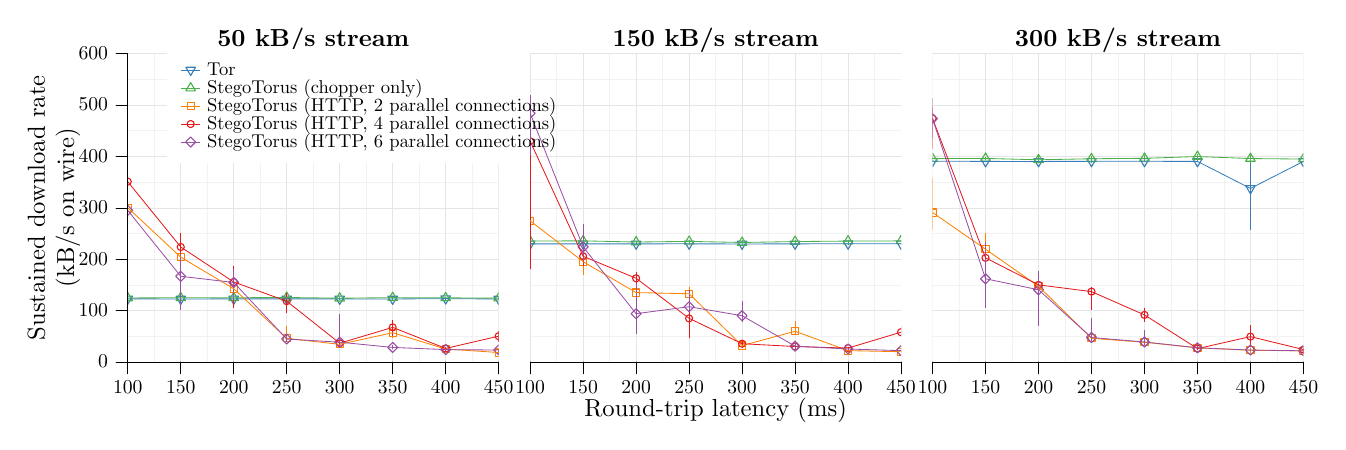
\begin{tikzpicture}[x=1pt,y=1pt]
\definecolor[named]{fillColor}{rgb}{1.00,1.00,1.00}
\begin{scope}
\path[clip] ( 38.09, 22.25) rectangle (172.12,133.66);
\definecolor[named]{drawColor}{rgb}{0.95,0.95,0.95}

\path[draw=drawColor,line width= 0.2pt,line join=round,line cap=round] ( 38.09, 31.54) --
	(172.12, 31.54);

\path[draw=drawColor,line width= 0.2pt,line join=round,line cap=round] ( 38.09, 50.11) --
	(172.12, 50.11);

\path[draw=drawColor,line width= 0.2pt,line join=round,line cap=round] ( 38.09, 68.67) --
	(172.12, 68.67);

\path[draw=drawColor,line width= 0.2pt,line join=round,line cap=round] ( 38.09, 87.24) --
	(172.12, 87.24);

\path[draw=drawColor,line width= 0.2pt,line join=round,line cap=round] ( 38.09,105.81) --
	(172.12,105.81);

\path[draw=drawColor,line width= 0.2pt,line join=round,line cap=round] ( 38.09,124.38) --
	(172.12,124.38);

\path[draw=drawColor,line width= 0.2pt,line join=round,line cap=round] ( 47.67, 22.25) --
	( 47.67,133.66);

\path[draw=drawColor,line width= 0.2pt,line join=round,line cap=round] ( 66.81, 22.25) --
	( 66.81,133.66);

\path[draw=drawColor,line width= 0.2pt,line join=round,line cap=round] ( 85.96, 22.25) --
	( 85.96,133.66);

\path[draw=drawColor,line width= 0.2pt,line join=round,line cap=round] (105.11, 22.25) --
	(105.11,133.66);

\path[draw=drawColor,line width= 0.2pt,line join=round,line cap=round] (124.25, 22.25) --
	(124.25,133.66);

\path[draw=drawColor,line width= 0.2pt,line join=round,line cap=round] (143.40, 22.25) --
	(143.40,133.66);

\path[draw=drawColor,line width= 0.2pt,line join=round,line cap=round] (162.54, 22.25) --
	(162.54,133.66);
\definecolor[named]{drawColor}{rgb}{0.90,0.90,0.90}

\path[draw=drawColor,line width= 0.2pt,line join=round,line cap=round] ( 38.09, 22.25) --
	(172.12, 22.25);

\path[draw=drawColor,line width= 0.2pt,line join=round,line cap=round] ( 38.09, 40.82) --
	(172.12, 40.82);

\path[draw=drawColor,line width= 0.2pt,line join=round,line cap=round] ( 38.09, 59.39) --
	(172.12, 59.39);

\path[draw=drawColor,line width= 0.2pt,line join=round,line cap=round] ( 38.09, 77.96) --
	(172.12, 77.96);

\path[draw=drawColor,line width= 0.2pt,line join=round,line cap=round] ( 38.09, 96.53) --
	(172.12, 96.53);

\path[draw=drawColor,line width= 0.2pt,line join=round,line cap=round] ( 38.09,115.10) --
	(172.12,115.10);

\path[draw=drawColor,line width= 0.2pt,line join=round,line cap=round] ( 38.09,133.66) --
	(172.12,133.66);

\path[draw=drawColor,line width= 0.2pt,line join=round,line cap=round] ( 38.09, 22.25) --
	( 38.09,133.66);

\path[draw=drawColor,line width= 0.2pt,line join=round,line cap=round] ( 57.24, 22.25) --
	( 57.24,133.66);

\path[draw=drawColor,line width= 0.2pt,line join=round,line cap=round] ( 76.39, 22.25) --
	( 76.39,133.66);

\path[draw=drawColor,line width= 0.2pt,line join=round,line cap=round] ( 95.53, 22.25) --
	( 95.53,133.66);

\path[draw=drawColor,line width= 0.2pt,line join=round,line cap=round] (114.68, 22.25) --
	(114.68,133.66);

\path[draw=drawColor,line width= 0.2pt,line join=round,line cap=round] (133.82, 22.25) --
	(133.82,133.66);

\path[draw=drawColor,line width= 0.2pt,line join=round,line cap=round] (152.97, 22.25) --
	(152.97,133.66);

\path[draw=drawColor,line width= 0.2pt,line join=round,line cap=round] (172.12, 22.25) --
	(172.12,133.66);
\definecolor[named]{drawColor}{rgb}{0.22,0.49,0.72}

\path[draw=drawColor,line width= 0.3pt,line join=round] ( 38.09, 44.80) -- ( 38.09, 45.15);

\path[draw=drawColor,line width= 0.3pt,line join=round] ( 57.24, 44.92) -- ( 57.24, 45.20);

\path[draw=drawColor,line width= 0.3pt,line join=round] ( 76.39, 45.05) -- ( 76.39, 45.10);

\path[draw=drawColor,line width= 0.3pt,line join=round] ( 95.53, 45.00) -- ( 95.53, 45.10);

\path[draw=drawColor,line width= 0.3pt,line join=round] (114.68, 45.01) -- (114.68, 45.13);

\path[draw=drawColor,line width= 0.3pt,line join=round] (133.82, 44.98) -- (133.82, 45.10);

\path[draw=drawColor,line width= 0.3pt,line join=round] (152.97, 44.86) -- (152.97, 45.14);

\path[draw=drawColor,line width= 0.3pt,line join=round] (172.12, 44.89) -- (172.12, 45.18);

\path[draw=drawColor,line width= 0.4pt,line join=round,line cap=round] ( 38.09, 43.07) --
	( 39.82, 46.05) --
	( 36.37, 46.05) --
	( 38.09, 43.07);

\path[draw=drawColor,line width= 0.4pt,line join=round,line cap=round] ( 57.24, 43.02) --
	( 58.96, 46.00) --
	( 55.52, 46.00) --
	( 57.24, 43.02);

\path[draw=drawColor,line width= 0.4pt,line join=round,line cap=round] ( 76.39, 43.05) --
	( 78.11, 46.04) --
	( 74.66, 46.04) --
	( 76.39, 43.05);

\path[draw=drawColor,line width= 0.4pt,line join=round,line cap=round] ( 95.53, 43.07) --
	( 97.26, 46.05) --
	( 93.81, 46.05) --
	( 95.53, 43.07);

\path[draw=drawColor,line width= 0.4pt,line join=round,line cap=round] (114.68, 43.05) --
	(116.40, 46.03) --
	(112.95, 46.03) --
	(114.68, 43.05);

\path[draw=drawColor,line width= 0.4pt,line join=round,line cap=round] (133.82, 43.02) --
	(135.55, 46.01) --
	(132.10, 46.01) --
	(133.82, 43.02);

\path[draw=drawColor,line width= 0.4pt,line join=round,line cap=round] (152.97, 43.14) --
	(154.70, 46.13) --
	(151.25, 46.13) --
	(152.97, 43.14);

\path[draw=drawColor,line width= 0.4pt,line join=round,line cap=round] (172.12, 43.01) --
	(173.84, 46.00) --
	(170.39, 46.00) --
	(172.12, 43.01);
\definecolor[named]{drawColor}{rgb}{0.30,0.69,0.29}

\path[draw=drawColor,line width= 0.3pt,line join=round] ( 38.09, 44.95) -- ( 38.09, 45.74);

\path[draw=drawColor,line width= 0.3pt,line join=round] ( 57.24, 45.32) -- ( 57.24, 45.70);

\path[draw=drawColor,line width= 0.3pt,line join=round] ( 76.39, 45.06) -- ( 76.39, 45.66);

\path[draw=drawColor,line width= 0.3pt,line join=round] ( 95.53, 45.17) -- ( 95.53, 45.66);

\path[draw=drawColor,line width= 0.3pt,line join=round] (114.68, 45.03) -- (114.68, 45.82);

\path[draw=drawColor,line width= 0.3pt,line join=round] (133.82, 44.90) -- (133.82, 45.70);

\path[draw=drawColor,line width= 0.3pt,line join=round] (152.97, 45.04) -- (152.97, 45.74);

\path[draw=drawColor,line width= 0.3pt,line join=round] (172.12, 45.04) -- (172.12, 45.65);

\path[draw=drawColor,line width= 0.4pt,line join=round,line cap=round] ( 38.09, 47.37) --
	( 39.82, 44.38) --
	( 36.37, 44.38) --
	( 38.09, 47.37);

\path[draw=drawColor,line width= 0.4pt,line join=round,line cap=round] ( 57.24, 47.44) --
	( 58.96, 44.46) --
	( 55.52, 44.46) --
	( 57.24, 47.44);

\path[draw=drawColor,line width= 0.4pt,line join=round,line cap=round] ( 76.39, 47.44) --
	( 78.11, 44.46) --
	( 74.66, 44.46) --
	( 76.39, 47.44);

\path[draw=drawColor,line width= 0.4pt,line join=round,line cap=round] ( 95.53, 47.54) --
	( 97.26, 44.55) --
	( 93.81, 44.55) --
	( 95.53, 47.54);

\path[draw=drawColor,line width= 0.4pt,line join=round,line cap=round] (114.68, 47.28) --
	(116.40, 44.29) --
	(112.95, 44.29) --
	(114.68, 47.28);

\path[draw=drawColor,line width= 0.4pt,line join=round,line cap=round] (133.82, 47.48) --
	(135.55, 44.49) --
	(132.10, 44.49) --
	(133.82, 47.48);

\path[draw=drawColor,line width= 0.4pt,line join=round,line cap=round] (152.97, 47.42) --
	(154.70, 44.44) --
	(151.25, 44.44) --
	(152.97, 47.42);

\path[draw=drawColor,line width= 0.4pt,line join=round,line cap=round] (172.12, 47.29) --
	(173.84, 44.30) --
	(170.39, 44.30) --
	(172.12, 47.29);
\definecolor[named]{drawColor}{rgb}{1.00,0.50,0.00}

\path[draw=drawColor,line width= 0.3pt,line join=round] ( 38.09, 63.49) -- ( 38.09, 95.04);

\path[draw=drawColor,line width= 0.3pt,line join=round] ( 57.24, 57.62) -- ( 57.24, 63.51);

\path[draw=drawColor,line width= 0.3pt,line join=round] ( 76.39, 46.69) -- ( 76.39, 52.70);

\path[draw=drawColor,line width= 0.3pt,line join=round] ( 95.53, 29.71) -- ( 95.53, 35.32);

\path[draw=drawColor,line width= 0.3pt,line join=round] (114.68, 28.31) -- (114.68, 29.79);

\path[draw=drawColor,line width= 0.3pt,line join=round] (133.82, 30.89) -- (133.82, 36.36);

\path[draw=drawColor,line width= 0.3pt,line join=round] (152.97, 26.24) -- (152.97, 27.43);

\path[draw=drawColor,line width= 0.3pt,line join=round] (172.12, 24.69) -- (172.12, 26.66);

\path[draw=drawColor,line width= 0.4pt,line join=round,line cap=round] ( 36.81, 76.71) rectangle ( 39.37, 79.27);

\path[draw=drawColor,line width= 0.4pt,line join=round,line cap=round] ( 55.96, 58.85) rectangle ( 58.52, 61.41);

\path[draw=drawColor,line width= 0.4pt,line join=round,line cap=round] ( 75.11, 47.43) rectangle ( 77.67, 49.99);

\path[draw=drawColor,line width= 0.4pt,line join=round,line cap=round] ( 94.25, 29.51) rectangle ( 96.81, 32.07);

\path[draw=drawColor,line width= 0.4pt,line join=round,line cap=round] (113.40, 27.34) rectangle (115.96, 29.90);

\path[draw=drawColor,line width= 0.4pt,line join=round,line cap=round] (132.54, 31.53) rectangle (135.10, 34.10);

\path[draw=drawColor,line width= 0.4pt,line join=round,line cap=round] (151.69, 25.66) rectangle (154.25, 28.22);

\path[draw=drawColor,line width= 0.4pt,line join=round,line cap=round] (170.84, 24.38) rectangle (173.40, 26.94);
\definecolor[named]{drawColor}{rgb}{0.89,0.10,0.11}

\path[draw=drawColor,line width= 0.3pt,line join=round] ( 38.09, 68.00) -- ( 38.09,104.32);

\path[draw=drawColor,line width= 0.3pt,line join=round] ( 57.24, 57.19) -- ( 57.24, 68.82);

\path[draw=drawColor,line width= 0.3pt,line join=round] ( 76.39, 41.83) -- ( 76.39, 56.80);

\path[draw=drawColor,line width= 0.3pt,line join=round] ( 95.53, 39.84) -- ( 95.53, 47.33);

\path[draw=drawColor,line width= 0.3pt,line join=round] (114.68, 27.62) -- (114.68, 30.08);

\path[draw=drawColor,line width= 0.3pt,line join=round] (133.82, 31.80) -- (133.82, 37.48);

\path[draw=drawColor,line width= 0.3pt,line join=round] (152.97, 26.45) -- (152.97, 27.50);

\path[draw=drawColor,line width= 0.3pt,line join=round] (172.12, 29.50) -- (172.12, 33.32);

\path[draw=drawColor,line width= 0.4pt,line join=round,line cap=round] ( 38.09, 87.40) circle (  1.28);

\path[draw=drawColor,line width= 0.4pt,line join=round,line cap=round] ( 57.24, 63.79) circle (  1.28);

\path[draw=drawColor,line width= 0.4pt,line join=round,line cap=round] ( 76.39, 51.15) circle (  1.28);

\path[draw=drawColor,line width= 0.4pt,line join=round,line cap=round] ( 95.53, 44.21) circle (  1.28);

\path[draw=drawColor,line width= 0.4pt,line join=round,line cap=round] (114.68, 29.02) circle (  1.28);

\path[draw=drawColor,line width= 0.4pt,line join=round,line cap=round] (133.82, 34.75) circle (  1.28);

\path[draw=drawColor,line width= 0.4pt,line join=round,line cap=round] (152.97, 27.14) circle (  1.28);

\path[draw=drawColor,line width= 0.4pt,line join=round,line cap=round] (172.12, 31.58) circle (  1.28);
\definecolor[named]{drawColor}{rgb}{0.60,0.31,0.64}

\path[draw=drawColor,line width= 0.3pt,line join=round] ( 38.09, 64.78) -- ( 38.09,105.02);

\path[draw=drawColor,line width= 0.3pt,line join=round] ( 57.24, 41.09) -- ( 57.24, 61.38);

\path[draw=drawColor,line width= 0.3pt,line join=round] ( 76.39, 44.95) -- ( 76.39, 55.95);

\path[draw=drawColor,line width= 0.3pt,line join=round] ( 95.53, 29.48) -- ( 95.53, 32.21);

\path[draw=drawColor,line width= 0.3pt,line join=round] (114.68, 28.49) -- (114.68, 39.75);

\path[draw=drawColor,line width= 0.3pt,line join=round] (133.82, 26.77) -- (133.82, 28.35);

\path[draw=drawColor,line width= 0.3pt,line join=round] (152.97, 26.39) -- (152.97, 27.51);

\path[draw=drawColor,line width= 0.3pt,line join=round] (172.12, 25.24) -- (172.12, 27.04);

\path[draw=drawColor,line width= 0.4pt,line join=round,line cap=round] ( 36.28, 77.01) --
	( 38.09, 78.82) --
	( 39.90, 77.01) --
	( 38.09, 75.20) --
	( 36.28, 77.01);

\path[draw=drawColor,line width= 0.4pt,line join=round,line cap=round] ( 55.43, 53.21) --
	( 57.24, 55.02) --
	( 59.05, 53.21) --
	( 57.24, 51.40) --
	( 55.43, 53.21);

\path[draw=drawColor,line width= 0.4pt,line join=round,line cap=round] ( 74.58, 50.97) --
	( 76.39, 52.78) --
	( 78.20, 50.97) --
	( 76.39, 49.16) --
	( 74.58, 50.97);

\path[draw=drawColor,line width= 0.4pt,line join=round,line cap=round] ( 93.72, 30.53) --
	( 95.53, 32.34) --
	( 97.34, 30.53) --
	( 95.53, 28.72) --
	( 93.72, 30.53);

\path[draw=drawColor,line width= 0.4pt,line join=round,line cap=round] (112.87, 29.39) --
	(114.68, 31.20) --
	(116.49, 29.39) --
	(114.68, 27.58) --
	(112.87, 29.39);

\path[draw=drawColor,line width= 0.4pt,line join=round,line cap=round] (132.01, 27.51) --
	(133.82, 29.32) --
	(135.64, 27.51) --
	(133.82, 25.70) --
	(132.01, 27.51);

\path[draw=drawColor,line width= 0.4pt,line join=round,line cap=round] (151.16, 26.71) --
	(152.97, 28.52) --
	(154.78, 26.71) --
	(152.97, 24.90) --
	(151.16, 26.71);

\path[draw=drawColor,line width= 0.4pt,line join=round,line cap=round] (170.31, 26.56) --
	(172.12, 28.37) --
	(173.93, 26.56) --
	(172.12, 24.75) --
	(170.31, 26.56);
\definecolor[named]{drawColor}{rgb}{0.22,0.49,0.72}

\path[draw=drawColor,line width= 0.3pt,line join=round] ( 38.09, 45.06) --
	( 57.24, 45.01) --
	( 76.39, 45.05) --
	( 95.53, 45.06) --
	(114.68, 45.04) --
	(133.82, 45.01) --
	(152.97, 45.13) --
	(172.12, 45.01);
\definecolor[named]{drawColor}{rgb}{0.30,0.69,0.29}

\path[draw=drawColor,line width= 0.3pt,line join=round] ( 38.09, 45.38) --
	( 57.24, 45.45) --
	( 76.39, 45.45) --
	( 95.53, 45.55) --
	(114.68, 45.29) --
	(133.82, 45.49) --
	(152.97, 45.43) --
	(172.12, 45.30);
\definecolor[named]{drawColor}{rgb}{1.00,0.50,0.00}

\path[draw=drawColor,line width= 0.3pt,line join=round] ( 38.09, 77.99) --
	( 57.24, 60.13) --
	( 76.39, 48.71) --
	( 95.53, 30.79) --
	(114.68, 28.62) --
	(133.82, 32.82) --
	(152.97, 26.94) --
	(172.12, 25.66);
\definecolor[named]{drawColor}{rgb}{0.89,0.10,0.11}

\path[draw=drawColor,line width= 0.3pt,line join=round] ( 38.09, 87.40) --
	( 57.24, 63.79) --
	( 76.39, 51.15) --
	( 95.53, 44.21) --
	(114.68, 29.02) --
	(133.82, 34.75) --
	(152.97, 27.14) --
	(172.12, 31.58);
\definecolor[named]{drawColor}{rgb}{0.60,0.31,0.64}

\path[draw=drawColor,line width= 0.3pt,line join=round] ( 38.09, 77.01) --
	( 57.24, 53.21) --
	( 76.39, 50.97) --
	( 95.53, 30.53) --
	(114.68, 29.39) --
	(133.82, 27.51) --
	(152.97, 26.71) --
	(172.12, 26.56);
\end{scope}
\begin{scope}
\path[clip] (183.50, 22.25) rectangle (317.52,133.66);
\definecolor[named]{drawColor}{rgb}{0.95,0.95,0.95}

\path[draw=drawColor,line width= 0.2pt,line join=round,line cap=round] (183.50, 31.54) --
	(317.52, 31.54);

\path[draw=drawColor,line width= 0.2pt,line join=round,line cap=round] (183.50, 50.11) --
	(317.52, 50.11);

\path[draw=drawColor,line width= 0.2pt,line join=round,line cap=round] (183.50, 68.67) --
	(317.52, 68.67);

\path[draw=drawColor,line width= 0.2pt,line join=round,line cap=round] (183.50, 87.24) --
	(317.52, 87.24);

\path[draw=drawColor,line width= 0.2pt,line join=round,line cap=round] (183.50,105.81) --
	(317.52,105.81);

\path[draw=drawColor,line width= 0.2pt,line join=round,line cap=round] (183.50,124.38) --
	(317.52,124.38);

\path[draw=drawColor,line width= 0.2pt,line join=round,line cap=round] (193.07, 22.25) --
	(193.07,133.66);

\path[draw=drawColor,line width= 0.2pt,line join=round,line cap=round] (212.22, 22.25) --
	(212.22,133.66);

\path[draw=drawColor,line width= 0.2pt,line join=round,line cap=round] (231.36, 22.25) --
	(231.36,133.66);

\path[draw=drawColor,line width= 0.2pt,line join=round,line cap=round] (250.51, 22.25) --
	(250.51,133.66);

\path[draw=drawColor,line width= 0.2pt,line join=round,line cap=round] (269.66, 22.25) --
	(269.66,133.66);

\path[draw=drawColor,line width= 0.2pt,line join=round,line cap=round] (288.80, 22.25) --
	(288.80,133.66);

\path[draw=drawColor,line width= 0.2pt,line join=round,line cap=round] (307.95, 22.25) --
	(307.95,133.66);
\definecolor[named]{drawColor}{rgb}{0.90,0.90,0.90}

\path[draw=drawColor,line width= 0.2pt,line join=round,line cap=round] (183.50, 22.25) --
	(317.52, 22.25);

\path[draw=drawColor,line width= 0.2pt,line join=round,line cap=round] (183.50, 40.82) --
	(317.52, 40.82);

\path[draw=drawColor,line width= 0.2pt,line join=round,line cap=round] (183.50, 59.39) --
	(317.52, 59.39);

\path[draw=drawColor,line width= 0.2pt,line join=round,line cap=round] (183.50, 77.96) --
	(317.52, 77.96);

\path[draw=drawColor,line width= 0.2pt,line join=round,line cap=round] (183.50, 96.53) --
	(317.52, 96.53);

\path[draw=drawColor,line width= 0.2pt,line join=round,line cap=round] (183.50,115.10) --
	(317.52,115.10);

\path[draw=drawColor,line width= 0.2pt,line join=round,line cap=round] (183.50,133.66) --
	(317.52,133.66);

\path[draw=drawColor,line width= 0.2pt,line join=round,line cap=round] (183.50, 22.25) --
	(183.50,133.66);

\path[draw=drawColor,line width= 0.2pt,line join=round,line cap=round] (202.64, 22.25) --
	(202.64,133.66);

\path[draw=drawColor,line width= 0.2pt,line join=round,line cap=round] (221.79, 22.25) --
	(221.79,133.66);

\path[draw=drawColor,line width= 0.2pt,line join=round,line cap=round] (240.94, 22.25) --
	(240.94,133.66);

\path[draw=drawColor,line width= 0.2pt,line join=round,line cap=round] (260.08, 22.25) --
	(260.08,133.66);

\path[draw=drawColor,line width= 0.2pt,line join=round,line cap=round] (279.23, 22.25) --
	(279.23,133.66);

\path[draw=drawColor,line width= 0.2pt,line join=round,line cap=round] (298.38, 22.25) --
	(298.38,133.66);

\path[draw=drawColor,line width= 0.2pt,line join=round,line cap=round] (317.52, 22.25) --
	(317.52,133.66);
\definecolor[named]{drawColor}{rgb}{0.22,0.49,0.72}

\path[draw=drawColor,line width= 0.3pt,line join=round] (183.50, 64.79) -- (183.50, 65.09);

\path[draw=drawColor,line width= 0.3pt,line join=round] (202.64, 64.71) -- (202.64, 65.09);

\path[draw=drawColor,line width= 0.3pt,line join=round] (221.79, 64.75) -- (221.79, 65.03);

\path[draw=drawColor,line width= 0.3pt,line join=round] (240.94, 64.87) -- (240.94, 65.06);

\path[draw=drawColor,line width= 0.3pt,line join=round] (260.08, 64.80) -- (260.08, 65.04);

\path[draw=drawColor,line width= 0.3pt,line join=round] (279.23, 64.80) -- (279.23, 64.97);

\path[draw=drawColor,line width= 0.3pt,line join=round] (298.38, 64.83) -- (298.38, 65.00);

\path[draw=drawColor,line width= 0.3pt,line join=round] (317.52, 64.79) -- (317.52, 65.01);

\path[draw=drawColor,line width= 0.4pt,line join=round,line cap=round] (183.50, 62.94) --
	(185.22, 65.93) --
	(181.77, 65.93) --
	(183.50, 62.94);

\path[draw=drawColor,line width= 0.4pt,line join=round,line cap=round] (202.64, 62.93) --
	(204.37, 65.92) --
	(200.92, 65.92) --
	(202.64, 62.93);

\path[draw=drawColor,line width= 0.4pt,line join=round,line cap=round] (221.79, 62.94) --
	(223.51, 65.92) --
	(220.07, 65.92) --
	(221.79, 62.94);

\path[draw=drawColor,line width= 0.4pt,line join=round,line cap=round] (240.94, 62.94) --
	(242.66, 65.93) --
	(239.21, 65.93) --
	(240.94, 62.94);

\path[draw=drawColor,line width= 0.4pt,line join=round,line cap=round] (260.08, 62.90) --
	(261.81, 65.89) --
	(258.36, 65.89) --
	(260.08, 62.90);

\path[draw=drawColor,line width= 0.4pt,line join=round,line cap=round] (279.23, 62.93) --
	(280.95, 65.92) --
	(277.50, 65.92) --
	(279.23, 62.93);

\path[draw=drawColor,line width= 0.4pt,line join=round,line cap=round] (298.38, 62.96) --
	(300.10, 65.95) --
	(296.65, 65.95) --
	(298.38, 62.96);

\path[draw=drawColor,line width= 0.4pt,line join=round,line cap=round] (317.52, 62.94) --
	(319.25, 65.93) --
	(315.80, 65.93) --
	(317.52, 62.94);
\definecolor[named]{drawColor}{rgb}{0.30,0.69,0.29}

\path[draw=drawColor,line width= 0.3pt,line join=round] (183.50, 65.81) -- (183.50, 66.29);

\path[draw=drawColor,line width= 0.3pt,line join=round] (202.64, 65.68) -- (202.64, 66.02);

\path[draw=drawColor,line width= 0.3pt,line join=round] (221.79, 65.03) -- (221.79, 66.00);

\path[draw=drawColor,line width= 0.3pt,line join=round] (240.94, 64.93) -- (240.94, 66.37);

\path[draw=drawColor,line width= 0.3pt,line join=round] (260.08, 65.09) -- (260.08, 66.43);

\path[draw=drawColor,line width= 0.3pt,line join=round] (279.23, 64.84) -- (279.23, 66.16);

\path[draw=drawColor,line width= 0.3pt,line join=round] (298.38, 65.29) -- (298.38, 66.16);

\path[draw=drawColor,line width= 0.3pt,line join=round] (317.52, 65.47) -- (317.52, 66.32);

\path[draw=drawColor,line width= 0.4pt,line join=round,line cap=round] (183.50, 67.95) --
	(185.22, 64.96) --
	(181.77, 64.96) --
	(183.50, 67.95);

\path[draw=drawColor,line width= 0.4pt,line join=round,line cap=round] (202.64, 68.00) --
	(204.37, 65.02) --
	(200.92, 65.02) --
	(202.64, 68.00);

\path[draw=drawColor,line width= 0.4pt,line join=round,line cap=round] (221.79, 67.58) --
	(223.51, 64.59) --
	(220.07, 64.59) --
	(221.79, 67.58);

\path[draw=drawColor,line width= 0.4pt,line join=round,line cap=round] (240.94, 67.81) --
	(242.66, 64.82) --
	(239.21, 64.82) --
	(240.94, 67.81);

\path[draw=drawColor,line width= 0.4pt,line join=round,line cap=round] (260.08, 67.41) --
	(261.81, 64.42) --
	(258.36, 64.42) --
	(260.08, 67.41);

\path[draw=drawColor,line width= 0.4pt,line join=round,line cap=round] (279.23, 67.76) --
	(280.95, 64.77) --
	(277.50, 64.77) --
	(279.23, 67.76);

\path[draw=drawColor,line width= 0.4pt,line join=round,line cap=round] (298.38, 67.93) --
	(300.10, 64.94) --
	(296.65, 64.94) --
	(298.38, 67.93);

\path[draw=drawColor,line width= 0.4pt,line join=round,line cap=round] (317.52, 67.99) --
	(319.25, 65.01) --
	(315.80, 65.01) --
	(317.52, 67.99);
\definecolor[named]{drawColor}{rgb}{1.00,0.50,0.00}

\path[draw=drawColor,line width= 0.3pt,line join=round] (183.50, 66.16) -- (183.50, 76.86);

\path[draw=drawColor,line width= 0.3pt,line join=round] (202.64, 53.79) -- (202.64, 62.43);

\path[draw=drawColor,line width= 0.3pt,line join=round] (221.79, 41.87) -- (221.79, 52.74);

\path[draw=drawColor,line width= 0.3pt,line join=round] (240.94, 39.80) -- (240.94, 49.26);

\path[draw=drawColor,line width= 0.3pt,line join=round] (260.08, 27.16) -- (260.08, 29.08);

\path[draw=drawColor,line width= 0.3pt,line join=round] (279.23, 32.44) -- (279.23, 36.91);

\path[draw=drawColor,line width= 0.3pt,line join=round] (298.38, 25.17) -- (298.38, 27.01);

\path[draw=drawColor,line width= 0.3pt,line join=round] (317.52, 25.50) -- (317.52, 26.62);

\path[draw=drawColor,line width= 0.4pt,line join=round,line cap=round] (182.22, 71.98) rectangle (184.78, 74.54);

\path[draw=drawColor,line width= 0.4pt,line join=round,line cap=round] (201.36, 57.20) rectangle (203.92, 59.76);

\path[draw=drawColor,line width= 0.4pt,line join=round,line cap=round] (220.51, 46.04) rectangle (223.07, 48.60);

\path[draw=drawColor,line width= 0.4pt,line join=round,line cap=round] (239.66, 45.62) rectangle (242.22, 48.18);

\path[draw=drawColor,line width= 0.4pt,line join=round,line cap=round] (258.80, 26.89) rectangle (261.36, 29.45);

\path[draw=drawColor,line width= 0.4pt,line join=round,line cap=round] (277.95, 32.06) rectangle (280.51, 34.62);

\path[draw=drawColor,line width= 0.4pt,line join=round,line cap=round] (297.10, 25.06) rectangle (299.66, 27.62);

\path[draw=drawColor,line width= 0.4pt,line join=round,line cap=round] (316.24, 24.67) rectangle (318.80, 27.24);
\definecolor[named]{drawColor}{rgb}{0.89,0.10,0.11}

\path[draw=drawColor,line width= 0.3pt,line join=round] (183.50, 55.78) -- (183.50,110.31);

\path[draw=drawColor,line width= 0.3pt,line join=round] (202.64, 57.01) -- (202.64, 67.80);

\path[draw=drawColor,line width= 0.3pt,line join=round] (221.79, 49.12) -- (221.79, 54.71);

\path[draw=drawColor,line width= 0.3pt,line join=round] (240.94, 30.78) -- (240.94, 43.36);

\path[draw=drawColor,line width= 0.3pt,line join=round] (260.08, 28.10) -- (260.08, 29.87);

\path[draw=drawColor,line width= 0.3pt,line join=round] (279.23, 26.44) -- (279.23, 28.46);

\path[draw=drawColor,line width= 0.3pt,line join=round] (298.38, 26.42) -- (298.38, 27.54);

\path[draw=drawColor,line width= 0.3pt,line join=round] (317.52, 31.82) -- (317.52, 35.42);

\path[draw=drawColor,line width= 0.4pt,line join=round,line cap=round] (183.50,102.02) circle (  1.28);

\path[draw=drawColor,line width= 0.4pt,line join=round,line cap=round] (202.64, 60.44) circle (  1.28);

\path[draw=drawColor,line width= 0.4pt,line join=round,line cap=round] (221.79, 52.48) circle (  1.28);

\path[draw=drawColor,line width= 0.4pt,line join=round,line cap=round] (240.94, 38.00) circle (  1.28);

\path[draw=drawColor,line width= 0.4pt,line join=round,line cap=round] (260.08, 28.85) circle (  1.28);

\path[draw=drawColor,line width= 0.4pt,line join=round,line cap=round] (279.23, 27.83) circle (  1.28);

\path[draw=drawColor,line width= 0.4pt,line join=round,line cap=round] (298.38, 27.27) circle (  1.28);

\path[draw=drawColor,line width= 0.4pt,line join=round,line cap=round] (317.52, 33.01) circle (  1.28);
\definecolor[named]{drawColor}{rgb}{0.60,0.31,0.64}

\path[draw=drawColor,line width= 0.3pt,line join=round] (183.50, 97.05) -- (183.50,118.64);

\path[draw=drawColor,line width= 0.3pt,line join=round] (202.64, 59.22) -- (202.64, 71.94);

\path[draw=drawColor,line width= 0.3pt,line join=round] (221.79, 32.37) -- (221.79, 50.66);

\path[draw=drawColor,line width= 0.3pt,line join=round] (240.94, 40.27) -- (240.94, 48.16);

\path[draw=drawColor,line width= 0.3pt,line join=round] (260.08, 36.57) -- (260.08, 44.35);

\path[draw=drawColor,line width= 0.3pt,line join=round] (279.23, 26.39) -- (279.23, 28.98);

\path[draw=drawColor,line width= 0.3pt,line join=round] (298.38, 26.09) -- (298.38, 27.21);

\path[draw=drawColor,line width= 0.3pt,line join=round] (317.52, 25.68) -- (317.52, 26.65);

\path[draw=drawColor,line width= 0.4pt,line join=round,line cap=round] (181.69,112.11) --
	(183.50,113.92) --
	(185.31,112.11) --
	(183.50,110.30) --
	(181.69,112.11);

\path[draw=drawColor,line width= 0.4pt,line join=round,line cap=round] (200.83, 63.84) --
	(202.64, 65.66) --
	(204.45, 63.84) --
	(202.64, 62.03) --
	(200.83, 63.84);

\path[draw=drawColor,line width= 0.4pt,line join=round,line cap=round] (219.98, 39.70) --
	(221.79, 41.51) --
	(223.60, 39.70) --
	(221.79, 37.89) --
	(219.98, 39.70);

\path[draw=drawColor,line width= 0.4pt,line join=round,line cap=round] (239.13, 42.21) --
	(240.94, 44.02) --
	(242.75, 42.21) --
	(240.94, 40.40) --
	(239.13, 42.21);

\path[draw=drawColor,line width= 0.4pt,line join=round,line cap=round] (258.27, 38.97) --
	(260.08, 40.78) --
	(261.89, 38.97) --
	(260.08, 37.16) --
	(258.27, 38.97);

\path[draw=drawColor,line width= 0.4pt,line join=round,line cap=round] (277.42, 27.97) --
	(279.23, 29.78) --
	(281.04, 27.97) --
	(279.23, 26.16) --
	(277.42, 27.97);

\path[draw=drawColor,line width= 0.4pt,line join=round,line cap=round] (296.56, 26.93) --
	(298.38, 28.75) --
	(300.19, 26.93) --
	(298.38, 25.12) --
	(296.56, 26.93);

\path[draw=drawColor,line width= 0.4pt,line join=round,line cap=round] (315.71, 26.34) --
	(317.52, 28.15) --
	(319.33, 26.34) --
	(317.52, 24.53) --
	(315.71, 26.34);
\definecolor[named]{drawColor}{rgb}{0.22,0.49,0.72}

\path[draw=drawColor,line width= 0.3pt,line join=round] (183.50, 64.93) --
	(202.64, 64.92) --
	(221.79, 64.93) --
	(240.94, 64.94) --
	(260.08, 64.89) --
	(279.23, 64.93) --
	(298.38, 64.95) --
	(317.52, 64.94);
\definecolor[named]{drawColor}{rgb}{0.30,0.69,0.29}

\path[draw=drawColor,line width= 0.3pt,line join=round] (183.50, 65.96) --
	(202.64, 66.01) --
	(221.79, 65.59) --
	(240.94, 65.82) --
	(260.08, 65.42) --
	(279.23, 65.76) --
	(298.38, 65.93) --
	(317.52, 66.00);
\definecolor[named]{drawColor}{rgb}{1.00,0.50,0.00}

\path[draw=drawColor,line width= 0.3pt,line join=round] (183.50, 73.26) --
	(202.64, 58.48) --
	(221.79, 47.32) --
	(240.94, 46.90) --
	(260.08, 28.17) --
	(279.23, 33.34) --
	(298.38, 26.34) --
	(317.52, 25.95);
\definecolor[named]{drawColor}{rgb}{0.89,0.10,0.11}

\path[draw=drawColor,line width= 0.3pt,line join=round] (183.50,102.02) --
	(202.64, 60.44) --
	(221.79, 52.48) --
	(240.94, 38.00) --
	(260.08, 28.85) --
	(279.23, 27.83) --
	(298.38, 27.27) --
	(317.52, 33.01);
\definecolor[named]{drawColor}{rgb}{0.60,0.31,0.64}

\path[draw=drawColor,line width= 0.3pt,line join=round] (183.50,112.11) --
	(202.64, 63.84) --
	(221.79, 39.70) --
	(240.94, 42.21) --
	(260.08, 38.97) --
	(279.23, 27.97) --
	(298.38, 26.93) --
	(317.52, 26.34);
\end{scope}
\begin{scope}
\path[clip] (328.90, 22.25) rectangle (462.93,133.66);
\definecolor[named]{drawColor}{rgb}{0.95,0.95,0.95}

\path[draw=drawColor,line width= 0.2pt,line join=round,line cap=round] (328.90, 31.54) --
	(462.93, 31.54);

\path[draw=drawColor,line width= 0.2pt,line join=round,line cap=round] (328.90, 50.11) --
	(462.93, 50.11);

\path[draw=drawColor,line width= 0.2pt,line join=round,line cap=round] (328.90, 68.67) --
	(462.93, 68.67);

\path[draw=drawColor,line width= 0.2pt,line join=round,line cap=round] (328.90, 87.24) --
	(462.93, 87.24);

\path[draw=drawColor,line width= 0.2pt,line join=round,line cap=round] (328.90,105.81) --
	(462.93,105.81);

\path[draw=drawColor,line width= 0.2pt,line join=round,line cap=round] (328.90,124.38) --
	(462.93,124.38);

\path[draw=drawColor,line width= 0.2pt,line join=round,line cap=round] (338.48, 22.25) --
	(338.48,133.66);

\path[draw=drawColor,line width= 0.2pt,line join=round,line cap=round] (357.62, 22.25) --
	(357.62,133.66);

\path[draw=drawColor,line width= 0.2pt,line join=round,line cap=round] (376.77, 22.25) --
	(376.77,133.66);

\path[draw=drawColor,line width= 0.2pt,line join=round,line cap=round] (395.91, 22.25) --
	(395.91,133.66);

\path[draw=drawColor,line width= 0.2pt,line join=round,line cap=round] (415.06, 22.25) --
	(415.06,133.66);

\path[draw=drawColor,line width= 0.2pt,line join=round,line cap=round] (434.21, 22.25) --
	(434.21,133.66);

\path[draw=drawColor,line width= 0.2pt,line join=round,line cap=round] (453.35, 22.25) --
	(453.35,133.66);
\definecolor[named]{drawColor}{rgb}{0.90,0.90,0.90}

\path[draw=drawColor,line width= 0.2pt,line join=round,line cap=round] (328.90, 22.25) --
	(462.93, 22.25);

\path[draw=drawColor,line width= 0.2pt,line join=round,line cap=round] (328.90, 40.82) --
	(462.93, 40.82);

\path[draw=drawColor,line width= 0.2pt,line join=round,line cap=round] (328.90, 59.39) --
	(462.93, 59.39);

\path[draw=drawColor,line width= 0.2pt,line join=round,line cap=round] (328.90, 77.96) --
	(462.93, 77.96);

\path[draw=drawColor,line width= 0.2pt,line join=round,line cap=round] (328.90, 96.53) --
	(462.93, 96.53);

\path[draw=drawColor,line width= 0.2pt,line join=round,line cap=round] (328.90,115.10) --
	(462.93,115.10);

\path[draw=drawColor,line width= 0.2pt,line join=round,line cap=round] (328.90,133.66) --
	(462.93,133.66);

\path[draw=drawColor,line width= 0.2pt,line join=round,line cap=round] (328.90, 22.25) --
	(328.90,133.66);

\path[draw=drawColor,line width= 0.2pt,line join=round,line cap=round] (348.05, 22.25) --
	(348.05,133.66);

\path[draw=drawColor,line width= 0.2pt,line join=round,line cap=round] (367.20, 22.25) --
	(367.20,133.66);

\path[draw=drawColor,line width= 0.2pt,line join=round,line cap=round] (386.34, 22.25) --
	(386.34,133.66);

\path[draw=drawColor,line width= 0.2pt,line join=round,line cap=round] (405.49, 22.25) --
	(405.49,133.66);

\path[draw=drawColor,line width= 0.2pt,line join=round,line cap=round] (424.63, 22.25) --
	(424.63,133.66);

\path[draw=drawColor,line width= 0.2pt,line join=round,line cap=round] (443.78, 22.25) --
	(443.78,133.66);

\path[draw=drawColor,line width= 0.2pt,line join=round,line cap=round] (462.93, 22.25) --
	(462.93,133.66);
\definecolor[named]{drawColor}{rgb}{0.22,0.49,0.72}

\path[draw=drawColor,line width= 0.3pt,line join=round] (328.90, 94.57) -- (328.90, 94.90);

\path[draw=drawColor,line width= 0.3pt,line join=round] (348.05, 94.55) -- (348.05, 94.99);

\path[draw=drawColor,line width= 0.3pt,line join=round] (367.20, 94.63) -- (367.20, 94.89);

\path[draw=drawColor,line width= 0.3pt,line join=round] (386.34, 94.61) -- (386.34, 94.84);

\path[draw=drawColor,line width= 0.3pt,line join=round] (405.49, 94.63) -- (405.49, 94.77);

\path[draw=drawColor,line width= 0.3pt,line join=round] (424.63, 94.60) -- (424.63, 94.86);

\path[draw=drawColor,line width= 0.3pt,line join=round] (443.78, 69.76) -- (443.78, 94.98);

\path[draw=drawColor,line width= 0.3pt,line join=round] (462.93, 94.56) -- (462.93, 94.92);

\path[draw=drawColor,line width= 0.4pt,line join=round,line cap=round] (328.90, 92.82) --
	(330.63, 95.80) --
	(327.18, 95.80) --
	(328.90, 92.82);

\path[draw=drawColor,line width= 0.4pt,line join=round,line cap=round] (348.05, 92.73) --
	(349.77, 95.71) --
	(346.32, 95.71) --
	(348.05, 92.73);

\path[draw=drawColor,line width= 0.4pt,line join=round,line cap=round] (367.20, 92.72) --
	(368.92, 95.71) --
	(365.47, 95.71) --
	(367.20, 92.72);

\path[draw=drawColor,line width= 0.4pt,line join=round,line cap=round] (386.34, 92.76) --
	(388.07, 95.75) --
	(384.62, 95.75) --
	(386.34, 92.76);

\path[draw=drawColor,line width= 0.4pt,line join=round,line cap=round] (405.49, 92.76) --
	(407.21, 95.75) --
	(403.76, 95.75) --
	(405.49, 92.76);

\path[draw=drawColor,line width= 0.4pt,line join=round,line cap=round] (424.63, 92.73) --
	(426.36, 95.72) --
	(422.91, 95.72) --
	(424.63, 92.73);

\path[draw=drawColor,line width= 0.4pt,line join=round,line cap=round] (443.78, 82.96) --
	(445.50, 85.95) --
	(442.06, 85.95) --
	(443.78, 82.96);

\path[draw=drawColor,line width= 0.4pt,line join=round,line cap=round] (462.93, 92.74) --
	(464.65, 95.72) --
	(461.20, 95.72) --
	(462.93, 92.74);
\definecolor[named]{drawColor}{rgb}{0.30,0.69,0.29}

\path[draw=drawColor,line width= 0.3pt,line join=round] (328.90, 94.92) -- (328.90, 96.58);

\path[draw=drawColor,line width= 0.3pt,line join=round] (348.05, 95.17) -- (348.05, 96.43);

\path[draw=drawColor,line width= 0.3pt,line join=round] (367.20, 94.59) -- (367.20, 96.59);

\path[draw=drawColor,line width= 0.3pt,line join=round] (386.34, 94.21) -- (386.34, 96.57);

\path[draw=drawColor,line width= 0.3pt,line join=round] (405.49, 94.99) -- (405.49, 97.18);

\path[draw=drawColor,line width= 0.3pt,line join=round] (424.63, 94.49) -- (424.63, 97.45);

\path[draw=drawColor,line width= 0.3pt,line join=round] (443.78, 93.98) -- (443.78, 96.95);

\path[draw=drawColor,line width= 0.3pt,line join=round] (462.93, 94.35) -- (462.93, 96.85);

\path[draw=drawColor,line width= 0.4pt,line join=round,line cap=round] (328.90, 97.72) --
	(330.63, 94.74) --
	(327.18, 94.74) --
	(328.90, 97.72);

\path[draw=drawColor,line width= 0.4pt,line join=round,line cap=round] (348.05, 97.79) --
	(349.77, 94.80) --
	(346.32, 94.80) --
	(348.05, 97.79);

\path[draw=drawColor,line width= 0.4pt,line join=round,line cap=round] (367.20, 97.29) --
	(368.92, 94.30) --
	(365.47, 94.30) --
	(367.20, 97.29);

\path[draw=drawColor,line width= 0.4pt,line join=round,line cap=round] (386.34, 97.67) --
	(388.07, 94.68) --
	(384.62, 94.68) --
	(386.34, 97.67);

\path[draw=drawColor,line width= 0.4pt,line join=round,line cap=round] (405.49, 97.82) --
	(407.21, 94.83) --
	(403.76, 94.83) --
	(405.49, 97.82);

\path[draw=drawColor,line width= 0.4pt,line join=round,line cap=round] (424.63, 98.48) --
	(426.36, 95.49) --
	(422.91, 95.49) --
	(424.63, 98.48);

\path[draw=drawColor,line width= 0.4pt,line join=round,line cap=round] (443.78, 97.74) --
	(445.50, 94.76) --
	(442.06, 94.76) --
	(443.78, 97.74);

\path[draw=drawColor,line width= 0.4pt,line join=round,line cap=round] (462.93, 97.56) --
	(464.65, 94.58) --
	(461.20, 94.58) --
	(462.93, 97.56);
\definecolor[named]{drawColor}{rgb}{1.00,0.50,0.00}

\path[draw=drawColor,line width= 0.3pt,line join=round] (328.90, 69.92) -- (328.90, 88.86);

\path[draw=drawColor,line width= 0.3pt,line join=round] (348.05, 54.33) -- (348.05, 68.83);

\path[draw=drawColor,line width= 0.3pt,line join=round] (367.20, 45.63) -- (367.20, 52.45);

\path[draw=drawColor,line width= 0.3pt,line join=round] (386.34, 30.09) -- (386.34, 33.56);

\path[draw=drawColor,line width= 0.3pt,line join=round] (405.49, 27.93) -- (405.49, 31.36);

\path[draw=drawColor,line width= 0.3pt,line join=round] (424.63, 26.52) -- (424.63, 27.85);

\path[draw=drawColor,line width= 0.3pt,line join=round] (443.78, 25.34) -- (443.78, 27.39);

\path[draw=drawColor,line width= 0.3pt,line join=round] (462.93, 25.26) -- (462.93, 26.52);

\path[draw=drawColor,line width= 0.4pt,line join=round,line cap=round] (327.62, 74.97) rectangle (330.18, 77.53);

\path[draw=drawColor,line width= 0.4pt,line join=round,line cap=round] (346.77, 61.71) rectangle (349.33, 64.27);

\path[draw=drawColor,line width= 0.4pt,line join=round,line cap=round] (365.91, 48.33) rectangle (368.48, 50.89);

\path[draw=drawColor,line width= 0.4pt,line join=round,line cap=round] (385.06, 29.52) rectangle (387.62, 32.08);

\path[draw=drawColor,line width= 0.4pt,line join=round,line cap=round] (404.21, 28.09) rectangle (406.77, 30.65);

\path[draw=drawColor,line width= 0.4pt,line join=round,line cap=round] (423.35, 26.07) rectangle (425.91, 28.63);

\path[draw=drawColor,line width= 0.4pt,line join=round,line cap=round] (442.50, 25.20) rectangle (445.06, 27.76);

\path[draw=drawColor,line width= 0.4pt,line join=round,line cap=round] (461.65, 24.97) rectangle (464.21, 27.53);
\definecolor[named]{drawColor}{rgb}{0.89,0.10,0.11}

\path[draw=drawColor,line width= 0.3pt,line join=round] (328.90, 99.26) -- (328.90,114.56);

\path[draw=drawColor,line width= 0.3pt,line join=round] (348.05, 54.60) -- (348.05, 65.44);

\path[draw=drawColor,line width= 0.3pt,line join=round] (367.20, 45.14) -- (367.20, 54.78);

\path[draw=drawColor,line width= 0.3pt,line join=round] (386.34, 40.97) -- (386.34, 49.34);

\path[draw=drawColor,line width= 0.3pt,line join=round] (405.49, 36.80) -- (405.49, 41.83);

\path[draw=drawColor,line width= 0.3pt,line join=round] (424.63, 26.54) -- (424.63, 28.40);

\path[draw=drawColor,line width= 0.3pt,line join=round] (443.78, 27.61) -- (443.78, 35.46);

\path[draw=drawColor,line width= 0.3pt,line join=round] (462.93, 25.30) -- (462.93, 27.17);

\path[draw=drawColor,line width= 0.4pt,line join=round,line cap=round] (328.90,110.24) circle (  1.28);

\path[draw=drawColor,line width= 0.4pt,line join=round,line cap=round] (348.05, 59.87) circle (  1.28);

\path[draw=drawColor,line width= 0.4pt,line join=round,line cap=round] (367.20, 50.11) circle (  1.28);

\path[draw=drawColor,line width= 0.4pt,line join=round,line cap=round] (386.34, 47.67) circle (  1.28);

\path[draw=drawColor,line width= 0.4pt,line join=round,line cap=round] (405.49, 39.25) circle (  1.28);

\path[draw=drawColor,line width= 0.4pt,line join=round,line cap=round] (424.63, 27.07) circle (  1.28);

\path[draw=drawColor,line width= 0.4pt,line join=round,line cap=round] (443.78, 31.41) circle (  1.28);

\path[draw=drawColor,line width= 0.4pt,line join=round,line cap=round] (462.93, 26.73) circle (  1.28);
\definecolor[named]{drawColor}{rgb}{0.60,0.31,0.64}

\path[draw=drawColor,line width= 0.3pt,line join=round] (328.90,103.11) -- (328.90,117.48);

\path[draw=drawColor,line width= 0.3pt,line join=round] (348.05, 41.88) -- (348.05, 65.62);

\path[draw=drawColor,line width= 0.3pt,line join=round] (367.20, 35.40) -- (367.20, 54.99);

\path[draw=drawColor,line width= 0.3pt,line join=round] (386.34, 29.73) -- (386.34, 38.18);

\path[draw=drawColor,line width= 0.3pt,line join=round] (405.49, 28.22) -- (405.49, 33.90);

\path[draw=drawColor,line width= 0.3pt,line join=round] (424.63, 26.98) -- (424.63, 28.14);

\path[draw=drawColor,line width= 0.3pt,line join=round] (443.78, 26.38) -- (443.78, 26.89);

\path[draw=drawColor,line width= 0.3pt,line join=round] (462.93, 25.47) -- (462.93, 27.25);

\path[draw=drawColor,line width= 0.4pt,line join=round,line cap=round] (327.09,110.17) --
	(328.90,111.98) --
	(330.71,110.17) --
	(328.90,108.36) --
	(327.09,110.17);

\path[draw=drawColor,line width= 0.4pt,line join=round,line cap=round] (346.24, 52.31) --
	(348.05, 54.12) --
	(349.86, 52.31) --
	(348.05, 50.50) --
	(346.24, 52.31);

\path[draw=drawColor,line width= 0.4pt,line join=round,line cap=round] (365.38, 48.34) --
	(367.20, 50.15) --
	(369.01, 48.34) --
	(367.20, 46.53) --
	(365.38, 48.34);

\path[draw=drawColor,line width= 0.4pt,line join=round,line cap=round] (384.53, 31.08) --
	(386.34, 32.89) --
	(388.15, 31.08) --
	(386.34, 29.27) --
	(384.53, 31.08);

\path[draw=drawColor,line width= 0.4pt,line join=round,line cap=round] (403.68, 29.47) --
	(405.49, 31.28) --
	(407.30, 29.47) --
	(405.49, 27.65) --
	(403.68, 29.47);

\path[draw=drawColor,line width= 0.4pt,line join=round,line cap=round] (422.82, 27.38) --
	(424.63, 29.19) --
	(426.44, 27.38) --
	(424.63, 25.57) --
	(422.82, 27.38);

\path[draw=drawColor,line width= 0.4pt,line join=round,line cap=round] (441.97, 26.55) --
	(443.78, 28.36) --
	(445.59, 26.55) --
	(443.78, 24.74) --
	(441.97, 26.55);

\path[draw=drawColor,line width= 0.4pt,line join=round,line cap=round] (461.12, 26.29) --
	(462.93, 28.10) --
	(464.74, 26.29) --
	(462.93, 24.48) --
	(461.12, 26.29);
\definecolor[named]{drawColor}{rgb}{0.22,0.49,0.72}

\path[draw=drawColor,line width= 0.3pt,line join=round] (328.90, 94.81) --
	(348.05, 94.72) --
	(367.20, 94.71) --
	(386.34, 94.75) --
	(405.49, 94.76) --
	(424.63, 94.72) --
	(443.78, 84.95) --
	(462.93, 94.73);
\definecolor[named]{drawColor}{rgb}{0.30,0.69,0.29}

\path[draw=drawColor,line width= 0.3pt,line join=round] (328.90, 95.73) --
	(348.05, 95.80) --
	(367.20, 95.30) --
	(386.34, 95.68) --
	(405.49, 95.83) --
	(424.63, 96.49) --
	(443.78, 95.75) --
	(462.93, 95.57);
\definecolor[named]{drawColor}{rgb}{1.00,0.50,0.00}

\path[draw=drawColor,line width= 0.3pt,line join=round] (328.90, 76.25) --
	(348.05, 62.99) --
	(367.20, 49.61) --
	(386.34, 30.80) --
	(405.49, 29.37) --
	(424.63, 27.35) --
	(443.78, 26.48) --
	(462.93, 26.25);
\definecolor[named]{drawColor}{rgb}{0.89,0.10,0.11}

\path[draw=drawColor,line width= 0.3pt,line join=round] (328.90,110.24) --
	(348.05, 59.87) --
	(367.20, 50.11) --
	(386.34, 47.67) --
	(405.49, 39.25) --
	(424.63, 27.07) --
	(443.78, 31.41) --
	(462.93, 26.73);
\definecolor[named]{drawColor}{rgb}{0.60,0.31,0.64}

\path[draw=drawColor,line width= 0.3pt,line join=round] (328.90,110.17) --
	(348.05, 52.31) --
	(367.20, 48.34) --
	(386.34, 31.08) --
	(405.49, 29.47) --
	(424.63, 27.38) --
	(443.78, 26.55) --
	(462.93, 26.29);
\end{scope}
\begin{scope}
\definecolor[named]{drawColor}{rgb}{0.00,0.00,0.00}

\node[text=drawColor,anchor=base,inner sep=0pt, outer sep=0pt, scale=  0.89] at (105.11,136.37) {\bfseries 50 kB/s stream};
\end{scope}
\begin{scope}
\definecolor[named]{drawColor}{rgb}{0.00,0.00,0.00}

\node[text=drawColor,anchor=base,inner sep=0pt, outer sep=0pt, scale=  0.89] at (250.51,136.37) {\bfseries 150 kB/s stream};
\end{scope}
\begin{scope}
\definecolor[named]{drawColor}{rgb}{0.00,0.00,0.00}

\node[text=drawColor,anchor=base,inner sep=0pt, outer sep=0pt, scale=  0.89] at (395.91,136.37) {\bfseries 300 kB/s stream};
\end{scope}
\begin{scope}
\definecolor[named]{drawColor}{rgb}{0.00,0.00,0.00}

\path[draw=drawColor,line width= 0.2pt,line join=round,line cap=round] ( 38.09, 22.25) -- ( 38.09,133.66);

\node[text=drawColor,anchor=base east,inner sep=0pt, outer sep=0pt, scale=  0.71] at ( 30.98, 20.09) {0};

\node[text=drawColor,anchor=base east,inner sep=0pt, outer sep=0pt, scale=  0.71] at ( 30.98, 38.66) {100};

\node[text=drawColor,anchor=base east,inner sep=0pt, outer sep=0pt, scale=  0.71] at ( 30.98, 57.23) {200};

\node[text=drawColor,anchor=base east,inner sep=0pt, outer sep=0pt, scale=  0.71] at ( 30.98, 75.80) {300};

\node[text=drawColor,anchor=base east,inner sep=0pt, outer sep=0pt, scale=  0.71] at ( 30.98, 94.37) {400};

\node[text=drawColor,anchor=base east,inner sep=0pt, outer sep=0pt, scale=  0.71] at ( 30.98,112.94) {500};

\node[text=drawColor,anchor=base east,inner sep=0pt, outer sep=0pt, scale=  0.71] at ( 30.98,131.50) {600};
\end{scope}
\begin{scope}
\definecolor[named]{drawColor}{rgb}{0.00,0.00,0.00}

\path[draw=drawColor,line width= 0.2pt,line join=round,line cap=round] ( 33.83, 22.25) -- ( 38.09, 22.25);

\path[draw=drawColor,line width= 0.2pt,line join=round,line cap=round] ( 33.83, 40.82) -- ( 38.09, 40.82);

\path[draw=drawColor,line width= 0.2pt,line join=round,line cap=round] ( 33.83, 59.39) -- ( 38.09, 59.39);

\path[draw=drawColor,line width= 0.2pt,line join=round,line cap=round] ( 33.83, 77.96) -- ( 38.09, 77.96);

\path[draw=drawColor,line width= 0.2pt,line join=round,line cap=round] ( 33.83, 96.53) -- ( 38.09, 96.53);

\path[draw=drawColor,line width= 0.2pt,line join=round,line cap=round] ( 33.83,115.10) -- ( 38.09,115.10);

\path[draw=drawColor,line width= 0.2pt,line join=round,line cap=round] ( 33.83,133.66) -- ( 38.09,133.66);
\end{scope}
\begin{scope}
\definecolor[named]{drawColor}{rgb}{0.00,0.00,0.00}

\path[draw=drawColor,line width= 0.2pt,line join=round,line cap=round] ( 38.09, 22.25) -- (172.12, 22.25);

\node[text=drawColor,anchor=base,inner sep=0pt, outer sep=0pt, scale=  0.71] at ( 38.09, 10.82) {100};

\node[text=drawColor,anchor=base,inner sep=0pt, outer sep=0pt, scale=  0.71] at ( 57.24, 10.82) {150};

\node[text=drawColor,anchor=base,inner sep=0pt, outer sep=0pt, scale=  0.71] at ( 76.39, 10.82) {200};

\node[text=drawColor,anchor=base,inner sep=0pt, outer sep=0pt, scale=  0.71] at ( 95.53, 10.82) {250};

\node[text=drawColor,anchor=base,inner sep=0pt, outer sep=0pt, scale=  0.71] at (114.68, 10.82) {300};

\node[text=drawColor,anchor=base,inner sep=0pt, outer sep=0pt, scale=  0.71] at (133.82, 10.82) {350};

\node[text=drawColor,anchor=base,inner sep=0pt, outer sep=0pt, scale=  0.71] at (152.97, 10.82) {400};

\node[text=drawColor,anchor=base,inner sep=0pt, outer sep=0pt, scale=  0.71] at (172.12, 10.82) {450};
\end{scope}
\begin{scope}
\definecolor[named]{drawColor}{rgb}{0.00,0.00,0.00}

\path[draw=drawColor,line width= 0.2pt,line join=round,line cap=round] ( 38.09, 17.99) -- ( 38.09, 22.25);

\path[draw=drawColor,line width= 0.2pt,line join=round,line cap=round] ( 57.24, 17.99) -- ( 57.24, 22.25);

\path[draw=drawColor,line width= 0.2pt,line join=round,line cap=round] ( 76.39, 17.99) -- ( 76.39, 22.25);

\path[draw=drawColor,line width= 0.2pt,line join=round,line cap=round] ( 95.53, 17.99) -- ( 95.53, 22.25);

\path[draw=drawColor,line width= 0.2pt,line join=round,line cap=round] (114.68, 17.99) -- (114.68, 22.25);

\path[draw=drawColor,line width= 0.2pt,line join=round,line cap=round] (133.82, 17.99) -- (133.82, 22.25);

\path[draw=drawColor,line width= 0.2pt,line join=round,line cap=round] (152.97, 17.99) -- (152.97, 22.25);

\path[draw=drawColor,line width= 0.2pt,line join=round,line cap=round] (172.12, 17.99) -- (172.12, 22.25);
\end{scope}
\begin{scope}
\definecolor[named]{drawColor}{rgb}{0.00,0.00,0.00}

\path[draw=drawColor,line width= 0.2pt,line join=round,line cap=round] (183.50, 22.25) -- (317.52, 22.25);

\node[text=drawColor,anchor=base,inner sep=0pt, outer sep=0pt, scale=  0.71] at (183.50, 10.82) {100};

\node[text=drawColor,anchor=base,inner sep=0pt, outer sep=0pt, scale=  0.71] at (202.64, 10.82) {150};

\node[text=drawColor,anchor=base,inner sep=0pt, outer sep=0pt, scale=  0.71] at (221.79, 10.82) {200};

\node[text=drawColor,anchor=base,inner sep=0pt, outer sep=0pt, scale=  0.71] at (240.94, 10.82) {250};

\node[text=drawColor,anchor=base,inner sep=0pt, outer sep=0pt, scale=  0.71] at (260.08, 10.82) {300};

\node[text=drawColor,anchor=base,inner sep=0pt, outer sep=0pt, scale=  0.71] at (279.23, 10.82) {350};

\node[text=drawColor,anchor=base,inner sep=0pt, outer sep=0pt, scale=  0.71] at (298.38, 10.82) {400};

\node[text=drawColor,anchor=base,inner sep=0pt, outer sep=0pt, scale=  0.71] at (317.52, 10.82) {450};
\end{scope}
\begin{scope}
\definecolor[named]{drawColor}{rgb}{0.00,0.00,0.00}

\path[draw=drawColor,line width= 0.2pt,line join=round,line cap=round] (183.50, 17.99) -- (183.50, 22.25);

\path[draw=drawColor,line width= 0.2pt,line join=round,line cap=round] (202.64, 17.99) -- (202.64, 22.25);

\path[draw=drawColor,line width= 0.2pt,line join=round,line cap=round] (221.79, 17.99) -- (221.79, 22.25);

\path[draw=drawColor,line width= 0.2pt,line join=round,line cap=round] (240.94, 17.99) -- (240.94, 22.25);

\path[draw=drawColor,line width= 0.2pt,line join=round,line cap=round] (260.08, 17.99) -- (260.08, 22.25);

\path[draw=drawColor,line width= 0.2pt,line join=round,line cap=round] (279.23, 17.99) -- (279.23, 22.25);

\path[draw=drawColor,line width= 0.2pt,line join=round,line cap=round] (298.38, 17.99) -- (298.38, 22.25);

\path[draw=drawColor,line width= 0.2pt,line join=round,line cap=round] (317.52, 17.99) -- (317.52, 22.25);
\end{scope}
\begin{scope}
\definecolor[named]{drawColor}{rgb}{0.00,0.00,0.00}

\path[draw=drawColor,line width= 0.2pt,line join=round,line cap=round] (328.90, 22.25) -- (462.93, 22.25);

\node[text=drawColor,anchor=base,inner sep=0pt, outer sep=0pt, scale=  0.71] at (328.90, 10.82) {100};

\node[text=drawColor,anchor=base,inner sep=0pt, outer sep=0pt, scale=  0.71] at (348.05, 10.82) {150};

\node[text=drawColor,anchor=base,inner sep=0pt, outer sep=0pt, scale=  0.71] at (367.20, 10.82) {200};

\node[text=drawColor,anchor=base,inner sep=0pt, outer sep=0pt, scale=  0.71] at (386.34, 10.82) {250};

\node[text=drawColor,anchor=base,inner sep=0pt, outer sep=0pt, scale=  0.71] at (405.49, 10.82) {300};

\node[text=drawColor,anchor=base,inner sep=0pt, outer sep=0pt, scale=  0.71] at (424.63, 10.82) {350};

\node[text=drawColor,anchor=base,inner sep=0pt, outer sep=0pt, scale=  0.71] at (443.78, 10.82) {400};

\node[text=drawColor,anchor=base,inner sep=0pt, outer sep=0pt, scale=  0.71] at (462.93, 10.82) {450};
\end{scope}
\begin{scope}
\definecolor[named]{drawColor}{rgb}{0.00,0.00,0.00}

\path[draw=drawColor,line width= 0.2pt,line join=round,line cap=round] (328.90, 17.99) -- (328.90, 22.25);

\path[draw=drawColor,line width= 0.2pt,line join=round,line cap=round] (348.05, 17.99) -- (348.05, 22.25);

\path[draw=drawColor,line width= 0.2pt,line join=round,line cap=round] (367.20, 17.99) -- (367.20, 22.25);

\path[draw=drawColor,line width= 0.2pt,line join=round,line cap=round] (386.34, 17.99) -- (386.34, 22.25);

\path[draw=drawColor,line width= 0.2pt,line join=round,line cap=round] (405.49, 17.99) -- (405.49, 22.25);

\path[draw=drawColor,line width= 0.2pt,line join=round,line cap=round] (424.63, 17.99) -- (424.63, 22.25);

\path[draw=drawColor,line width= 0.2pt,line join=round,line cap=round] (443.78, 17.99) -- (443.78, 22.25);

\path[draw=drawColor,line width= 0.2pt,line join=round,line cap=round] (462.93, 17.99) -- (462.93, 22.25);
\end{scope}
\begin{scope}
\definecolor[named]{drawColor}{rgb}{0.00,0.00,0.00}

\node[text=drawColor,anchor=base,inner sep=0pt, outer sep=0pt, scale=  0.89] at (250.51,  2.71) {Round-trip latency (ms)};
\end{scope}
\begin{scope}
\definecolor[named]{drawColor}{rgb}{0.00,0.00,0.00}

\node[text=drawColor,rotate= 90.00,anchor=base,inner sep=0pt, outer sep=0pt, scale=  0.89] at (  8.11, 77.96) {Sustained download rate};

\node[text=drawColor,rotate= 90.00,anchor=base,inner sep=0pt, outer sep=0pt, scale=  0.89] at ( 18.67, 77.96) {(kB/s on wire)};
\end{scope}
\begin{scope}
\definecolor[named]{fillColor}{rgb}{1.00,1.00,1.00}

\path[fill=fillColor] ( 52.23, 94.20) rectangle (176.90,135.25);
\end{scope}
\begin{scope}
\definecolor[named]{drawColor}{rgb}{0.22,0.49,0.72}

\path[draw=drawColor,line width= 0.3pt,line join=round] ( 57.36,127.73) -- ( 64.30,127.73);

\path[draw=drawColor,line width= 0.4pt,line join=round,line cap=round] ( 60.83,125.74) --
	( 62.56,128.73) --
	( 59.11,128.73) --
	( 60.83,125.74);
\end{scope}
\begin{scope}
\definecolor[named]{drawColor}{rgb}{0.22,0.49,0.72}

\path[draw=drawColor,line width= 0.3pt,line join=round] ( 57.36,127.73) -- ( 64.30,127.73);
\end{scope}
\begin{scope}
\definecolor[named]{drawColor}{rgb}{0.30,0.69,0.29}

\path[draw=drawColor,line width= 0.3pt,line join=round] ( 57.36,121.23) -- ( 64.30,121.23);

\path[draw=drawColor,line width= 0.4pt,line join=round,line cap=round] ( 60.83,123.22) --
	( 62.56,120.23) --
	( 59.11,120.23) --
	( 60.83,123.22);
\end{scope}
\begin{scope}
\definecolor[named]{drawColor}{rgb}{0.30,0.69,0.29}

\path[draw=drawColor,line width= 0.3pt,line join=round] ( 57.36,121.23) -- ( 64.30,121.23);
\end{scope}
\begin{scope}
\definecolor[named]{drawColor}{rgb}{1.00,0.50,0.00}

\path[draw=drawColor,line width= 0.3pt,line join=round] ( 57.36,114.72) -- ( 64.30,114.72);

\path[draw=drawColor,line width= 0.4pt,line join=round,line cap=round] ( 59.55,113.44) rectangle ( 62.11,116.00);
\end{scope}
\begin{scope}
\definecolor[named]{drawColor}{rgb}{1.00,0.50,0.00}

\path[draw=drawColor,line width= 0.3pt,line join=round] ( 57.36,114.72) -- ( 64.30,114.72);
\end{scope}
\begin{scope}
\definecolor[named]{drawColor}{rgb}{0.89,0.10,0.11}

\path[draw=drawColor,line width= 0.3pt,line join=round] ( 57.36,108.22) -- ( 64.30,108.22);

\path[draw=drawColor,line width= 0.4pt,line join=round,line cap=round] ( 60.83,108.22) circle (  1.28);
\end{scope}
\begin{scope}
\definecolor[named]{drawColor}{rgb}{0.89,0.10,0.11}

\path[draw=drawColor,line width= 0.3pt,line join=round] ( 57.36,108.22) -- ( 64.30,108.22);
\end{scope}
\begin{scope}
\definecolor[named]{drawColor}{rgb}{0.60,0.31,0.64}

\path[draw=drawColor,line width= 0.3pt,line join=round] ( 57.36,101.72) -- ( 64.30,101.72);

\path[draw=drawColor,line width= 0.4pt,line join=round,line cap=round] ( 59.02,101.72) --
	( 60.83,103.53) --
	( 62.64,101.72) --
	( 60.83, 99.90) --
	( 59.02,101.72);
\end{scope}
\begin{scope}
\definecolor[named]{drawColor}{rgb}{0.60,0.31,0.64}

\path[draw=drawColor,line width= 0.3pt,line join=round] ( 57.36,101.72) -- ( 64.30,101.72);
\end{scope}
\begin{scope}
\definecolor[named]{drawColor}{rgb}{0.00,0.00,0.00}

\node[text=drawColor,anchor=base west,inner sep=0pt, outer sep=0pt, scale=  0.67] at ( 66.80,125.71) {Tor};
\end{scope}
\begin{scope}
\definecolor[named]{drawColor}{rgb}{0.00,0.00,0.00}

\node[text=drawColor,anchor=base west,inner sep=0pt, outer sep=0pt, scale=  0.67] at ( 66.80,119.20) {StegoTorus (chopper only)};
\end{scope}
\begin{scope}
\definecolor[named]{drawColor}{rgb}{0.00,0.00,0.00}

\node[text=drawColor,anchor=base west,inner sep=0pt, outer sep=0pt, scale=  0.67] at ( 66.80,112.70) {StegoTorus (HTTP, 2 parallel connections)};
\end{scope}
\begin{scope}
\definecolor[named]{drawColor}{rgb}{0.00,0.00,0.00}

\node[text=drawColor,anchor=base west,inner sep=0pt, outer sep=0pt, scale=  0.67] at ( 66.80,106.19) {StegoTorus (HTTP, 4 parallel connections)};
\end{scope}
\begin{scope}
\definecolor[named]{drawColor}{rgb}{0.00,0.00,0.00}

\node[text=drawColor,anchor=base west,inner sep=0pt, outer sep=0pt, scale=  0.67] at ( 66.80, 99.69) {StegoTorus (HTTP, 6 parallel connections)};
\end{scope}
\end{tikzpicture}

\caption{Overhead and resilience of StegoTorus' \textit{HTTP}
  steganography module, compared to Tor alone and to StegoTorus in
  chopper-only operation.  Each data point shows median bandwidth
  consumption over a 20-second interval while transferring a
  continuous, fixed-rate stream of traffic over a 5.6~Mbps DSL link
  with adjustable latency.  Whiskers indicate the inter-hinge
  distance~\cite{s-boxplot}.  Tor and chopper-only StegoTorus do not
  suffer from latencies up to at least 450~ms.  The present
  \textit{HTTP} module is much more sensitive to latency, and cannot
  keep up with high-bandwidth streams at higher
  latencies.}\label{f:resilience}
\end{figure*}

An AUC score of 0.5 indicates a classifier performing no better than
random guessing, and a score of 1 indicates perfect accuracy.
Over Tor by itself, we can often obtain AUC scores better than 0.95,
but over StegoTorus, the scores drop to 0.75 or less in most cases.
For real-time classification of the traffic volume seen at a perimeter
router, the adversary requires an AUC score very close to 1 to avoid
being swamped by errors.  StegoTorus does not reduce the adversary's
odds all the way to chance, but it reduces them far enough to make the
attack impractical.

A determined adversary might train additional classifiers on visits to
sites of interest \emph{over StegoTorus}.  However, these classifiers
will be dependent on the covertext database that the adversary used
for training, so StegoTorus users who generate their own covertext
databases will be protected from this tactic.

\section{Performance}\label{s:peval}

All performance tests were conducted using a desktop PC in California
with a DSL link to the Internet (\Mbps{5.6} down, \Mbps{0.7} up) as the
client, and a virtual host in a commercial data center in New
Jersey as the server.  During testing, the DSL link was otherwise
idle, and round-trip latency between the two machines was \msec{85}.  To
ensure that our results reflect the performance of StegoTorus itself
rather than factors beyond our control (such as the instantaneous load
on the global Tor network), we configured a private Tor network
entirely within the server host, and sourced all of the test files and
streams from an HTTP server also running on that host.

\smallskip\noindent\textbf{Steganographic Expansion:} We performed a
series of downloads of 1,000,000-byte files and measured the amount of
data actually transferred over the network by a direct HTTP
connection, Tor, StegoTorus using the chopper alone, and StegoTorus
with the \textit{HTTP} module. The results are shown in
Table~\ref{t:expansion}.  Tor itself has a small amount of overhead,
and the chopper imposes a little bit more, but HTTP steganography is
very expensive by comparison, increasing the amount of data sent
upstream by a factor of 41, and downstream by 12.  While we have not
spent much time on optimizing our encoding, an expansion factor of at
least eight (one byte per bit) is typical for modern steganography
schemes~\cite{a-stat-steg}, so we suspect that HTTP steganography
cannot be made \emph{that} much more efficient in the downstream
direction.

\begin{table}[ht!]
\centering\small
\newcommand\z{\phantom{.0}}
\begin{tabular}{lr@{\hspace{6pt}}rr@{\hspace{6pt}}r}
\toprule
&\multicolumn{2}{c}{\textbf{To server}}&%
 \multicolumn{2}{c}{\textbf{From server}}\\
&\textbf{bytes}&$\boldsymbol{\times}$&\textbf{bytes}&$\boldsymbol{\times}$\\
\midrule
Direct               &  23,643 &  1\z &  1,014,401 &  1\z \\
Tor                  &  61,162 &  2.6 &  1,075,715 &  1.1 \\
StegoTorus (chopper) &  63,061 &  2.7 &  1,084,228 &  1.1 \\
StegoTorus (HTTP)    & 966,964 & 41\z & 11,814,610 & 12\z \\
\bottomrule
\end{tabular}
\caption{Mean number of bytes transferred in each direction in order
  to download a 1,000,000-byte file directly, over Tor, and over
  StegoTorus with and without HTTP steganography.  The file was
  downloaded 32 times for each test.}
\label{t:expansion}
\end{table}

\begin{figure}[ht!]
\centering
% Created by tikzDevice version GitHub Dev on 2012-08-10 11:58:54
% !TEX encoding = UTF-8 Unicode
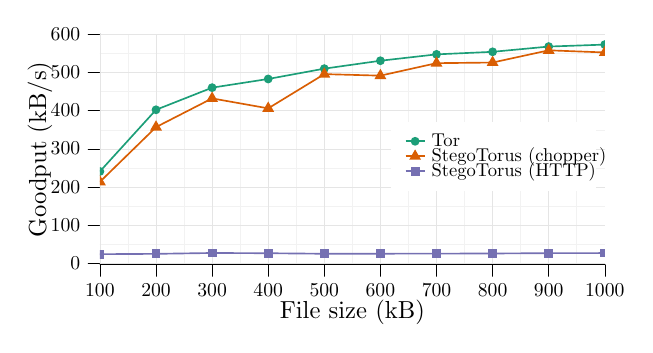
\begin{tikzpicture}[x=1pt,y=1pt]
\definecolor[named]{fillColor}{rgb}{1.00,1.00,1.00}
\begin{scope}
\definecolor[named]{drawColor}{rgb}{0.00,0.00,0.00}

\path[draw=drawColor,line width= 0.2pt,line join=round,line cap=round] ( 27.53, 22.25) -- ( 27.53,105.56);

\node[text=drawColor,anchor=base east,inner sep=0pt, outer sep=0pt, scale=  0.71] at ( 20.42, 20.48) {0};

\node[text=drawColor,anchor=base east,inner sep=0pt, outer sep=0pt, scale=  0.71] at ( 20.42, 34.29) {100};

\node[text=drawColor,anchor=base east,inner sep=0pt, outer sep=0pt, scale=  0.71] at ( 20.42, 48.09) {200};

\node[text=drawColor,anchor=base east,inner sep=0pt, outer sep=0pt, scale=  0.71] at ( 20.42, 61.89) {300};

\node[text=drawColor,anchor=base east,inner sep=0pt, outer sep=0pt, scale=  0.71] at ( 20.42, 75.70) {400};

\node[text=drawColor,anchor=base east,inner sep=0pt, outer sep=0pt, scale=  0.71] at ( 20.42, 89.50) {500};

\node[text=drawColor,anchor=base east,inner sep=0pt, outer sep=0pt, scale=  0.71] at ( 20.42,103.31) {600};
\end{scope}
\begin{scope}
\definecolor[named]{drawColor}{rgb}{0.00,0.00,0.00}

\path[draw=drawColor,line width= 0.2pt,line join=round,line cap=round] ( 23.27, 22.64) -- ( 27.53, 22.64);

\path[draw=drawColor,line width= 0.2pt,line join=round,line cap=round] ( 23.27, 36.45) -- ( 27.53, 36.45);

\path[draw=drawColor,line width= 0.2pt,line join=round,line cap=round] ( 23.27, 50.25) -- ( 27.53, 50.25);

\path[draw=drawColor,line width= 0.2pt,line join=round,line cap=round] ( 23.27, 64.05) -- ( 27.53, 64.05);

\path[draw=drawColor,line width= 0.2pt,line join=round,line cap=round] ( 23.27, 77.86) -- ( 27.53, 77.86);

\path[draw=drawColor,line width= 0.2pt,line join=round,line cap=round] ( 23.27, 91.66) -- ( 27.53, 91.66);

\path[draw=drawColor,line width= 0.2pt,line join=round,line cap=round] ( 23.27,105.47) -- ( 27.53,105.47);
\end{scope}
\begin{scope}
\path[clip] ( 27.53, 22.25) rectangle (209.98,105.56);
\definecolor[named]{drawColor}{rgb}{0.95,0.95,0.95}

\path[draw=drawColor,line width= 0.2pt,line join=round,line cap=round] ( 27.53, 29.54) --
	(209.98, 29.54);

\path[draw=drawColor,line width= 0.2pt,line join=round,line cap=round] ( 27.53, 43.35) --
	(209.98, 43.35);

\path[draw=drawColor,line width= 0.2pt,line join=round,line cap=round] ( 27.53, 57.15) --
	(209.98, 57.15);

\path[draw=drawColor,line width= 0.2pt,line join=round,line cap=round] ( 27.53, 70.96) --
	(209.98, 70.96);

\path[draw=drawColor,line width= 0.2pt,line join=round,line cap=round] ( 27.53, 84.76) --
	(209.98, 84.76);

\path[draw=drawColor,line width= 0.2pt,line join=round,line cap=round] ( 27.53, 98.57) --
	(209.98, 98.57);

\path[draw=drawColor,line width= 0.2pt,line join=round,line cap=round] ( 37.67, 22.25) --
	( 37.67,105.56);

\path[draw=drawColor,line width= 0.2pt,line join=round,line cap=round] ( 57.94, 22.25) --
	( 57.94,105.56);

\path[draw=drawColor,line width= 0.2pt,line join=round,line cap=round] ( 78.21, 22.25) --
	( 78.21,105.56);

\path[draw=drawColor,line width= 0.2pt,line join=round,line cap=round] ( 98.49, 22.25) --
	( 98.49,105.56);

\path[draw=drawColor,line width= 0.2pt,line join=round,line cap=round] (118.76, 22.25) --
	(118.76,105.56);

\path[draw=drawColor,line width= 0.2pt,line join=round,line cap=round] (139.03, 22.25) --
	(139.03,105.56);

\path[draw=drawColor,line width= 0.2pt,line join=round,line cap=round] (159.30, 22.25) --
	(159.30,105.56);

\path[draw=drawColor,line width= 0.2pt,line join=round,line cap=round] (179.57, 22.25) --
	(179.57,105.56);

\path[draw=drawColor,line width= 0.2pt,line join=round,line cap=round] (199.85, 22.25) --
	(199.85,105.56);
\definecolor[named]{drawColor}{rgb}{0.90,0.90,0.90}

\path[draw=drawColor,line width= 0.2pt,line join=round,line cap=round] ( 27.53, 22.64) --
	(209.98, 22.64);

\path[draw=drawColor,line width= 0.2pt,line join=round,line cap=round] ( 27.53, 36.45) --
	(209.98, 36.45);

\path[draw=drawColor,line width= 0.2pt,line join=round,line cap=round] ( 27.53, 50.25) --
	(209.98, 50.25);

\path[draw=drawColor,line width= 0.2pt,line join=round,line cap=round] ( 27.53, 64.05) --
	(209.98, 64.05);

\path[draw=drawColor,line width= 0.2pt,line join=round,line cap=round] ( 27.53, 77.86) --
	(209.98, 77.86);

\path[draw=drawColor,line width= 0.2pt,line join=round,line cap=round] ( 27.53, 91.66) --
	(209.98, 91.66);

\path[draw=drawColor,line width= 0.2pt,line join=round,line cap=round] ( 27.53,105.47) --
	(209.98,105.47);

\path[draw=drawColor,line width= 0.2pt,line join=round,line cap=round] ( 27.53, 22.25) --
	( 27.53,105.56);

\path[draw=drawColor,line width= 0.2pt,line join=round,line cap=round] ( 47.81, 22.25) --
	( 47.81,105.56);

\path[draw=drawColor,line width= 0.2pt,line join=round,line cap=round] ( 68.08, 22.25) --
	( 68.08,105.56);

\path[draw=drawColor,line width= 0.2pt,line join=round,line cap=round] ( 88.35, 22.25) --
	( 88.35,105.56);

\path[draw=drawColor,line width= 0.2pt,line join=round,line cap=round] (108.62, 22.25) --
	(108.62,105.56);

\path[draw=drawColor,line width= 0.2pt,line join=round,line cap=round] (128.89, 22.25) --
	(128.89,105.56);

\path[draw=drawColor,line width= 0.2pt,line join=round,line cap=round] (149.17, 22.25) --
	(149.17,105.56);

\path[draw=drawColor,line width= 0.2pt,line join=round,line cap=round] (169.44, 22.25) --
	(169.44,105.56);

\path[draw=drawColor,line width= 0.2pt,line join=round,line cap=round] (189.71, 22.25) --
	(189.71,105.56);

\path[draw=drawColor,line width= 0.2pt,line join=round,line cap=round] (209.98, 22.25) --
	(209.98,105.56);
\definecolor[named]{drawColor}{rgb}{0.11,0.62,0.47}

\path[draw=drawColor,line width= 0.6pt,line join=round] ( 27.53, 55.93) --
	( 47.81, 78.21) --
	( 68.08, 86.21) --
	( 88.35, 89.35) --
	(108.62, 93.08) --
	(128.89, 95.94) --
	(149.17, 98.24) --
	(169.44, 99.16) --
	(189.71,101.06) --
	(209.98,101.77);
\definecolor[named]{drawColor}{rgb}{0.85,0.37,0.01}

\path[draw=drawColor,line width= 0.6pt,line join=round] ( 27.53, 52.17) --
	( 47.81, 71.95) --
	( 68.08, 82.33) --
	( 88.35, 78.73) --
	(108.62, 91.10) --
	(128.89, 90.55) --
	(149.17, 95.06) --
	(169.44, 95.29) --
	(189.71, 99.70) --
	(209.98, 98.93);
\definecolor[named]{drawColor}{rgb}{0.46,0.44,0.70}

\path[draw=drawColor,line width= 0.6pt,line join=round] ( 27.53, 26.04) --
	( 47.81, 26.16) --
	( 68.08, 26.47) --
	( 88.35, 26.38) --
	(108.62, 26.19) --
	(128.89, 26.22) --
	(149.17, 26.23) --
	(169.44, 26.29) --
	(189.71, 26.40) --
	(209.98, 26.44);
\definecolor[named]{fillColor}{rgb}{0.11,0.62,0.47}

\path[fill=fillColor] ( 27.53, 55.93) circle (  1.60);

\path[fill=fillColor] ( 47.81, 78.21) circle (  1.60);

\path[fill=fillColor] ( 68.08, 86.21) circle (  1.60);

\path[fill=fillColor] ( 88.35, 89.35) circle (  1.60);

\path[fill=fillColor] (108.62, 93.08) circle (  1.60);

\path[fill=fillColor] (128.89, 95.94) circle (  1.60);

\path[fill=fillColor] (149.17, 98.24) circle (  1.60);

\path[fill=fillColor] (169.44, 99.16) circle (  1.60);

\path[fill=fillColor] (189.71,101.06) circle (  1.60);

\path[fill=fillColor] (209.98,101.77) circle (  1.60);
\definecolor[named]{fillColor}{rgb}{0.85,0.37,0.01}

\path[fill=fillColor] ( 27.53, 54.65) --
	( 29.69, 50.92) --
	( 25.38, 50.92) --
	cycle;

\path[fill=fillColor] ( 47.81, 74.44) --
	( 49.96, 70.71) --
	( 45.65, 70.71) --
	cycle;

\path[fill=fillColor] ( 68.08, 84.82) --
	( 70.23, 81.09) --
	( 65.92, 81.09) --
	cycle;

\path[fill=fillColor] ( 88.35, 81.22) --
	( 90.50, 77.49) --
	( 86.19, 77.49) --
	cycle;

\path[fill=fillColor] (108.62, 93.59) --
	(110.78, 89.85) --
	(106.47, 89.85) --
	cycle;

\path[fill=fillColor] (128.89, 93.04) --
	(131.05, 89.30) --
	(126.74, 89.30) --
	cycle;

\path[fill=fillColor] (149.17, 97.55) --
	(151.32, 93.81) --
	(147.01, 93.81) --
	cycle;

\path[fill=fillColor] (169.44, 97.78) --
	(171.59, 94.05) --
	(167.28, 94.05) --
	cycle;

\path[fill=fillColor] (189.71,102.18) --
	(191.86, 98.45) --
	(187.55, 98.45) --
	cycle;

\path[fill=fillColor] (209.98,101.42) --
	(212.14, 97.69) --
	(207.83, 97.69) --
	cycle;
\definecolor[named]{fillColor}{rgb}{0.46,0.44,0.70}

\path[fill=fillColor] ( 25.93, 24.44) --
	( 29.13, 24.44) --
	( 29.13, 27.64) --
	( 25.93, 27.64) --
	cycle;

\path[fill=fillColor] ( 46.20, 24.56) --
	( 49.41, 24.56) --
	( 49.41, 27.76) --
	( 46.20, 27.76) --
	cycle;

\path[fill=fillColor] ( 66.48, 24.87) --
	( 69.68, 24.87) --
	( 69.68, 28.07) --
	( 66.48, 28.07) --
	cycle;

\path[fill=fillColor] ( 86.75, 24.78) --
	( 89.95, 24.78) --
	( 89.95, 27.98) --
	( 86.75, 27.98) --
	cycle;

\path[fill=fillColor] (107.02, 24.59) --
	(110.22, 24.59) --
	(110.22, 27.79) --
	(107.02, 27.79) --
	cycle;

\path[fill=fillColor] (127.29, 24.62) --
	(130.49, 24.62) --
	(130.49, 27.83) --
	(127.29, 27.83) --
	cycle;

\path[fill=fillColor] (147.56, 24.63) --
	(150.77, 24.63) --
	(150.77, 27.83) --
	(147.56, 27.83) --
	cycle;

\path[fill=fillColor] (167.84, 24.69) --
	(171.04, 24.69) --
	(171.04, 27.89) --
	(167.84, 27.89) --
	cycle;

\path[fill=fillColor] (188.11, 24.80) --
	(191.31, 24.80) --
	(191.31, 28.00) --
	(188.11, 28.00) --
	cycle;

\path[fill=fillColor] (208.38, 24.84) --
	(211.58, 24.84) --
	(211.58, 28.04) --
	(208.38, 28.04) --
	cycle;
\end{scope}
\begin{scope}
\definecolor[named]{drawColor}{rgb}{0.00,0.00,0.00}

\path[draw=drawColor,line width= 0.2pt,line join=round,line cap=round] ( 27.53, 22.25) -- (209.98, 22.25);

\node[text=drawColor,anchor=base,inner sep=0pt, outer sep=0pt, scale=  0.71] at ( 27.53, 10.82) {100};

\node[text=drawColor,anchor=base,inner sep=0pt, outer sep=0pt, scale=  0.71] at ( 47.81, 10.82) {200};

\node[text=drawColor,anchor=base,inner sep=0pt, outer sep=0pt, scale=  0.71] at ( 68.08, 10.82) {300};

\node[text=drawColor,anchor=base,inner sep=0pt, outer sep=0pt, scale=  0.71] at ( 88.35, 10.82) {400};

\node[text=drawColor,anchor=base,inner sep=0pt, outer sep=0pt, scale=  0.71] at (108.62, 10.82) {500};

\node[text=drawColor,anchor=base,inner sep=0pt, outer sep=0pt, scale=  0.71] at (128.89, 10.82) {600};

\node[text=drawColor,anchor=base,inner sep=0pt, outer sep=0pt, scale=  0.71] at (149.17, 10.82) {700};

\node[text=drawColor,anchor=base,inner sep=0pt, outer sep=0pt, scale=  0.71] at (169.44, 10.82) {800};

\node[text=drawColor,anchor=base,inner sep=0pt, outer sep=0pt, scale=  0.71] at (189.71, 10.82) {900};

\node[text=drawColor,anchor=base,inner sep=0pt, outer sep=0pt, scale=  0.71] at (209.98, 10.82) {1000};
\end{scope}
\begin{scope}
\definecolor[named]{drawColor}{rgb}{0.00,0.00,0.00}

\path[draw=drawColor,line width= 0.2pt,line join=round,line cap=round] ( 27.53, 17.99) -- ( 27.53, 22.25);

\path[draw=drawColor,line width= 0.2pt,line join=round,line cap=round] ( 47.81, 17.99) -- ( 47.81, 22.25);

\path[draw=drawColor,line width= 0.2pt,line join=round,line cap=round] ( 68.08, 17.99) -- ( 68.08, 22.25);

\path[draw=drawColor,line width= 0.2pt,line join=round,line cap=round] ( 88.35, 17.99) -- ( 88.35, 22.25);

\path[draw=drawColor,line width= 0.2pt,line join=round,line cap=round] (108.62, 17.99) -- (108.62, 22.25);

\path[draw=drawColor,line width= 0.2pt,line join=round,line cap=round] (128.89, 17.99) -- (128.89, 22.25);

\path[draw=drawColor,line width= 0.2pt,line join=round,line cap=round] (149.17, 17.99) -- (149.17, 22.25);

\path[draw=drawColor,line width= 0.2pt,line join=round,line cap=round] (169.44, 17.99) -- (169.44, 22.25);

\path[draw=drawColor,line width= 0.2pt,line join=round,line cap=round] (189.71, 17.99) -- (189.71, 22.25);

\path[draw=drawColor,line width= 0.2pt,line join=round,line cap=round] (209.98, 17.99) -- (209.98, 22.25);
\end{scope}
\begin{scope}
\definecolor[named]{drawColor}{rgb}{0.00,0.00,0.00}

\node[text=drawColor,anchor=base,inner sep=0pt, outer sep=0pt, scale=  0.89] at (118.76,  2.71) {File size (kB)};
\end{scope}
\begin{scope}
\definecolor[named]{drawColor}{rgb}{0.00,0.00,0.00}

\node[text=drawColor,rotate= 90.00,anchor=base,inner sep=0pt, outer sep=0pt, scale=  0.89] at (  8.11, 63.91) {Goodput (kB/s)};
\end{scope}
\begin{scope}
\definecolor[named]{fillColor}{rgb}{1.00,1.00,1.00}

\path[fill=fillColor] (132.84, 49.01) rectangle (206.85, 73.81);
\end{scope}
\begin{scope}
\definecolor[named]{drawColor}{rgb}{0.11,0.62,0.47}

\path[draw=drawColor,line width= 0.6pt,line join=round] (137.98, 66.83) -- (144.91, 66.83);
\end{scope}
\begin{scope}
\definecolor[named]{fillColor}{rgb}{0.11,0.62,0.47}

\path[fill=fillColor] (141.44, 66.83) circle (  1.60);
\end{scope}
\begin{scope}
\definecolor[named]{drawColor}{rgb}{0.85,0.37,0.01}

\path[draw=drawColor,line width= 0.6pt,line join=round] (137.98, 61.41) -- (144.91, 61.41);
\end{scope}
\begin{scope}
\definecolor[named]{fillColor}{rgb}{0.85,0.37,0.01}

\path[fill=fillColor] (141.44, 63.90) --
	(143.60, 60.16) --
	(139.29, 60.16) --
	cycle;
\end{scope}
\begin{scope}
\definecolor[named]{drawColor}{rgb}{0.46,0.44,0.70}

\path[draw=drawColor,line width= 0.6pt,line join=round] (137.98, 55.99) -- (144.91, 55.99);
\end{scope}
\begin{scope}
\definecolor[named]{fillColor}{rgb}{0.46,0.44,0.70}

\path[fill=fillColor] (139.84, 54.39) --
	(143.04, 54.39) --
	(143.04, 57.59) --
	(139.84, 57.59) --
	cycle;
\end{scope}
\begin{scope}
\definecolor[named]{drawColor}{rgb}{0.00,0.00,0.00}

\node[text=drawColor,anchor=base west,inner sep=0pt, outer sep=0pt, scale=  0.67] at (147.41, 64.80) {Tor};
\end{scope}
\begin{scope}
\definecolor[named]{drawColor}{rgb}{0.00,0.00,0.00}

\node[text=drawColor,anchor=base west,inner sep=0pt, outer sep=0pt, scale=  0.67] at (147.41, 59.38) {StegoTorus (chopper)};
\end{scope}
\begin{scope}
\definecolor[named]{drawColor}{rgb}{0.00,0.00,0.00}

\node[text=drawColor,anchor=base west,inner sep=0pt, outer sep=0pt, scale=  0.67] at (147.41, 53.96) {StegoTorus (HTTP)};
\end{scope}
\end{tikzpicture}

\caption{Mean StegoTorus (ST) and Tor goodput for \SI{100}{\kilo\byte}
  to \SI{1}{\mega\byte} file transfers.}\label{f:goodput}
\end{figure}

\smallskip\noindent\textbf{Goodput:} Expanding on the previous
experiment, we conducted more downloads of files of various sizes,
measured the time required, and computed the mean goodput (that is,
application-layer throughput) achieved in the same configurations
described earlier; the results are shown in Figure~\ref{f:goodput}.
We see that the goodput of the chopper-only configuration is
comparable to Tor, and that StegoTorus-HTTP is only able to achieve
goodput of roughly \kBps{27}, which is still about 4 times better than
a \kbps{56} modem.  Consistent with this, we have been able to use
StegoTorus-HTTP as-is for casual Web browsing; subjectively speaking,
it is noticeably slower than a direct broadband connection, but not so
slow that waiting for page loads becomes tedious.

\smallskip\noindent\textbf{Resilience:} Since StegoTorus may be used
in locations with poor connectivity, we also investigated its
performance as a function of network latency.  We used Linux's
\textit{netem} mechanism~\cite{s-netem} to vary the round-trip latency
to the StegoTorus server from \SIrange{100}{450}{\milli\second}.  For
comparison, packets from California take approximately \msec{85} to
reach New Jersey, \SIrange{120}{180}{\milli\second} to reach East Asia or
Australia, and \SIrange{300}{350}{\milli\second} to reach India or Africa.

We configured the server to generate continuous streams of data at
three different rates, thus measuring steady-state behavior, and
recorded the median bandwidth consumption over a period of 20 seconds
at each latency setting.  The results are shown in
Figure~\ref{f:resilience}.  Ideal behavior would be for each line to
be perfectly horizontal, and as close to the “Tor” line as possible.

Both Tor and StegoTorus in chopper-only mode are robust up to
\msec{450} of delay, suffering no measurable performance degradation.
The \textit{HTTP} module, however, can keep up with a \kBps{50} data
stream only at latencies below \msec{200}.  Allowing \textit{HTTP} to
use more parallel connections increases throughput at low latencies,
but does not help it keep up at high latencies.  We suspect this is
because each chopper block, which typically will only contain one or
two Tor cells, takes a full HTTP request-response pair to transfer to
the peer.  Thus we are only transferring one or two Tor cells per
round-trip cycle, despite consuming far more bandwidth.  However, we
believe that the \textit{HTTP} module can be improved to handle high
latency at least somewhat better, and plan to make this a priority for
future work.

\section{Previous Work}\label{s:prev-work}

The earliest academic study of Internet censorship we are aware of is
a~\citeyear{richardson2002us.health} case study of porn-blocking
“filters” used in schools and libraries in the
USA~\cite{richardson2002us.health}.  Its authors were concerned that
these filters might misclassify sexual health information as
pornographic.  To check, they manually compiled a set of health- and
porn-related keywords, expanded it to a list of 4,000 URLs by
searching the Web without any filters active (2,500 URLs were
health-related, 500 pornographic, and 1,000 neither) and then
attempted to visit all of the pages with filters in place.

This methodology---probing the behavior of a filter with keyword
searches, specific URLs known to contain sensitive content, or
both---is still standard for censorship case studies.  China has
received the most attention~\cite{clayton2006cn.ignore,
  park2010cn.filter, xu2011cn.where, anderson2012cn.splinternet,
  wright2014cn.regional}. Similar studies have been published for
Iran~\cite{aryan2013ir.first}, Pakistan~\cite{nabi2013pk.anatomy,
  nabi2014.futile}, and Turkey~\cite{nabi2014.futile}.  The OpenNet
Initiative (ONI) regularly surveys roughly 80 countries
worldwide~\cite{oni.nd.profiles, oni2008denied, oni2010controlled}.

The same methodology also underlies broader studies.  One line of
research investigates inter-country variation in the censorship
\emph{mechanism}: for instance, whether censorship mainly interferes
with DNS lookups or subsequent TCP connections, and whether the
end-user is informed of censorship~\cite{verkamp2012.mechanics}. In
some cases, it has been possible to identify the specific “filter” in
use~\cite{dalek2013.url.filtering, jones.2014.blockpages}. Another
line aims to understand what is censored and
why~\cite{aase2012whiskey}, how that changes over
time~\cite{anderson2014.ripe,gill.2015.worldwide}, how the degree of
censorship might vary within a country~\cite{wright2011.finegrain},
and how people react to
censorship~\cite{khattak.2014.isp,knockel.2011.skype}.

Despite the central position of keyword and URL probe lists in all of
these studies, relatively little attention has been paid to the
contents of the lists, or how they are developed.  Far more effort has
gone into refining the methodology of the probes
themselves~\cite{dalek2013.url.filtering, dischinger2010.diffserv,
  filasto2012.ooni, jones.2014.blockpages, sfakianakis2011.censmon,
  wright2011.finegrain, verkamp2012.mechanics, burnett2015.encore}.
A few studies have dug into “leaks” of inside information, which allow
researchers to see what actually \emph{is} censored and perhaps why.
Recently this has occurred for backbone filters in
Syria~\cite{chaabane.2014.syria} and Pakistan~\cite{khattak.2014.isp},
and the TOM-Skype chat client's internal keyword
filter~\cite{knockel.2011.skype}.  However, all of these studies still
took the list as a means to an end, not an object of research in
itself.

One notable exception, and the effort closest to our own research, is
the ConceptDoppler project~\cite{crandall2007.conceptdoppler}.  The
authors attempted to refine a keyword list, using latent semantic
analysis to generate new keywords from a “seed set” of
known-filtered keywords.  Their goal was to develop a system that
could track the time evolution of a keyword blacklist in real time, so
that it could be correlated with news events.  While their initial
results were promising, the algorithm required a great deal of manual
validation and adjustment, and we are not aware of any follow-up work.

\section{Conclusion}\label{s:conclusion}
We described StegoTorus, a new system for improving Tor's robustness
against automated protocol analysis.  StegoTorus interposes on
communications between the Tor client and the first Tor relay,
implements a custom encryption protocol and provides a suite of
steganography modules that make Tor resilient to fingerprinting
attacks.  Our statistical evaluations demonstrate that StegoTorus
makes Tor traffic more resilient to site fingerprinting attacks and
and that it resembles HTTP in the dimensions of connection length,
payload size and bandwidth use.  Our performance measurements indicate
that our prototype system, in its HTTP steganography mode, delivers
throughput of roughly \kBps{30}, which is about four times that of a
\kbps{56} modem.

\smallskip\noindent\textbf{Future Work:} There is much room for
further research on expanding and strengthening our suite of
steganography modules.  Beyond steganography modules we plan to
explore opportunities for performance improvements and add support for
redundant coding among steganography modules.

\section{Acknowledgments}

We appreciate helpful comments during system and paper development
from Arjun Athreya, Brian Caswell, Drew Dean, Bruce DeBruhl,
Roger Dingledine, Pamela Griffith, David-Sarah Hopwood,
George Kadianakis, Eric Kline, Patrick Lincoln, Nick Mathewson,
Phil Porras, Steve Schwab, William Allen Simpson, Paul Vixie,
and Mike Walker.
Paul Hick and kc claffy at CAIDA~\cite{d-caida} provided access to
anonymized backbone traces.  Data analysis was done in R~\cite{s-r}
with the “ggplot2” plotting add-on~\cite{s-ggplot2}.

This material is based on work supported by the Defense Advanced
Research Project Agency (DARPA) and Space and Naval Warfare Systems
Center Pacific under Contract No.\ N66001-11-C-4022, and by a National
Science Foundation Graduate Research Fellowship under Grant
No.\ DGE-1147470.  Any opinions, findings, conclusions, or
recommendations expressed in this material are those of the authors,
and do not necessarily reflect the views of the Defense Advanced
Research Project Agency, Space and Naval Warfare Systems Center
Pacific, or the National Science Foundation.  Distribution Statement
“A:” Approved for Public Release, Distribution Unlimited.


\bibliography{stegotorus}

\end{document}
% Local Variables:
% mode: latex
% encoding: utf-8
% End:
